\chapter{Search for Displaced Vertices}
\label{sec:vertexing}
The HPS vertexing search is a low-background search for heavy photons with displaced vertices.
This search is sensitive to heavy photons with low coupling, and therefore low production but long decay lengths.

The pair selection for the vertexing search requires cuts in addition to the basic cuts described in Section \ref{sec:event_selection}.
These vertex quality cuts are tuned to suppress the tails of the vertex distribution, and are described in Section \ref{sec:vertex_cuts}.

\begin{figure}[ht]
\begin{center}
    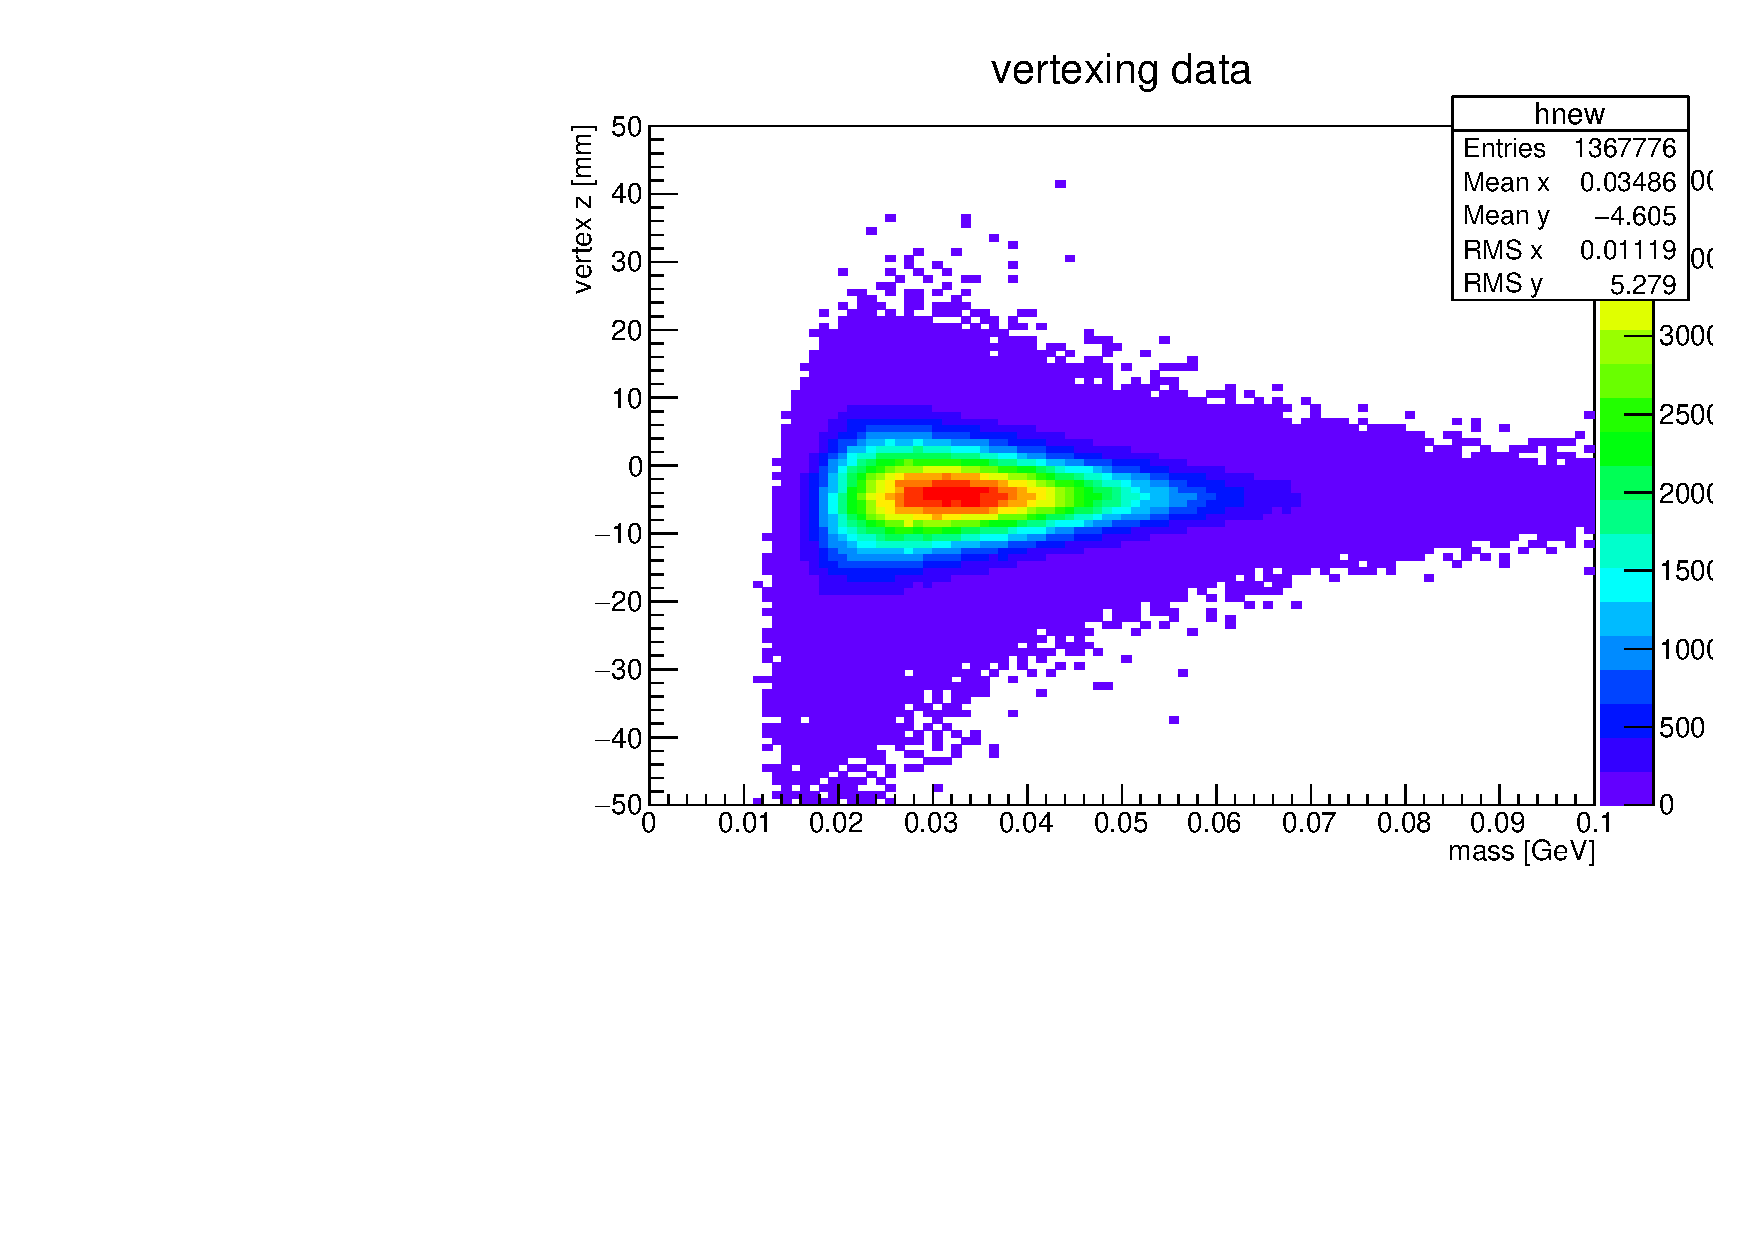
\includegraphics[width=0.7\textwidth,page=1,angle=-90]{vertexing/figs/golden_mres}
\end{center}
    \caption{Dataset for the vertexing analysis. The core of the vertex distribution is the horizontal band at $z=-5$ mm; a heavy photon signal would appear as a vertical band extending upwards from the core.}
    \label{fig:zvsmass}
\end{figure}

The pairs passing cuts are reduced to a 2-D dataset of points $(m,z)$, where each point is the mass $m$ and vertex location $z$ of a pair: see Figure \ref{fig:zvsmass}.
The vertex $z$ is the distance along the HPS beam axis, and is defined relative to the nominal target position; as explained in Section \ref{sec:target_z}, the actual target position is at $z_{target}\approx -5$ mm.
To test for a heavy photon with $m_{A'}=m$, a resolution-limited mass slice ($|m-m_{A'}|<1.4\sigma_m$) is taken from the 2-D data set, and the vertex $z$ of the pairs in this mass slice are plotted as in Figure \ref{fig:vz_1d}.

\begin{figure}[ht]
\begin{center}
    \includegraphics[width=0.7\textwidth,page=61,angle=-90]{vertexing/figs/golden_mres}
\end{center}
\caption{Vertex $z$ (units of mm) for a resolution-limited mass slice (in data) centered at $m_{A'}=35.5$ MeV. A heavy photon signal would appear as a low-level tail extending to higher $z$ (longer than the exponential tail of the blue curve, which is the prompt vertex distribution described in Section \ref{sec:tails}).
    For this mass slice, $z_{cut}=26.6$ mm; there are four events with $z>z_{cut}$.}
    \label{fig:vz_1d}
\end{figure}

A cut is made at a minimum $z>z_{cut}$ to remove the large background from prompt $e^+e^-$ pairs.
$z_{cut}$ (plotted in Figure \ref{fig:zcut}) is set so the expected number of events past $z_{cut}$ is 0.5 according to a model of the prompt pairs distribution, described in Section \ref{sec:tails}.
This minimizes the prompt backgrounds and maximizes the heavy photon signal.
The rectangular region formed by the mass and $z$ cuts is the signal box for the heavy photon with mass $m_{A'}$.

If a heavy photon exists at some $m_{A'}$, heavy photon decays will appear in the data with a Gaussian mass distribution centered at $m_{A'}$, and a distribution of locations that extend from $z_{target}$ to positive $z$.
These events will appear in those mass slices that are close enough to $m_{A'}$ that they substantially overlap the Gaussian.

\begin{figure}[ht]
\begin{center}
    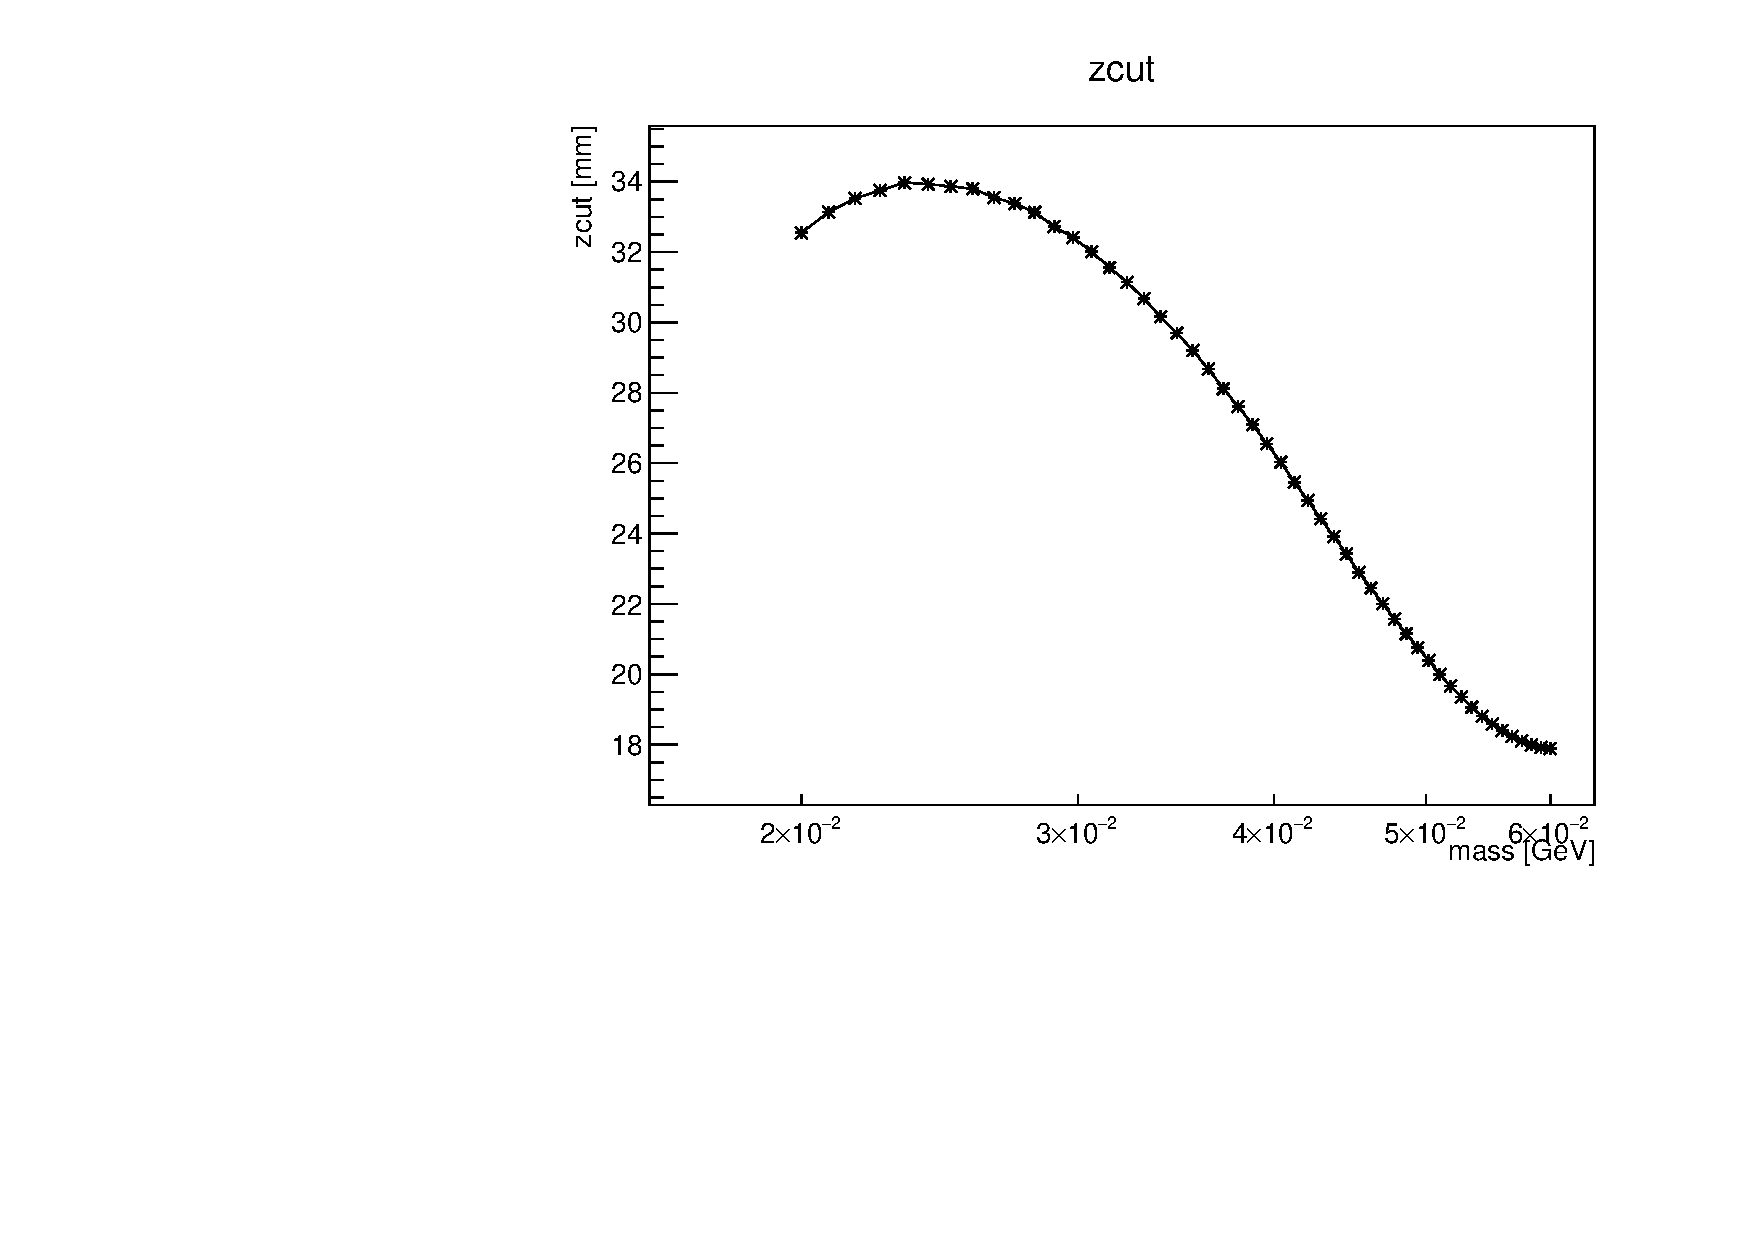
\includegraphics[width=0.7\textwidth,page=1,angle=-90]{vertexing/figs/golden_mres_output}
\end{center}
\caption{The value of the cut $z>z_{cut}$, as a function of the center of the mass slice.
The number of events per mass slice decreases and the $z$ resolution improves as the mass increases; both effects tend to reduce $z_{cut}$.}
    \label{fig:zcut}
\end{figure}

Two types of analyses are performed on the data in the signal box.
The first is a cut-and-count analysis, where the number of pairs found in the signal box is compared to the number expected; this analysis gives the significance of any observed excess over background, and is described in Section \ref{sec:significance}.
The second analysis uses the optimum interval method to set an upper limit on the heavy photon production rate, and is described in Section \ref{sec:limits}.

\clearpage
\section{Heavy Photon Monte Carlo}
\label{sec:ap_mc}
Heavy photon Monte Carlo samples are generated for values of $m_{A'}$ spaced out across the region of interest: 15, 16, 17, 18, 19, 20, 22, 24, 26, 28, 30, 35, 40, 50, 60, 70, 80, and 90 MeV.
The generator is similar to those described in Section \ref{sec:tri_mc}.
It uses MadGraph/MadEvent, and fully simulates the momentum and angle spectra of the produced heavy photons.
In order to get complete coverage of $z>z_{target}$ for the purposes of the vertexing analysis, the decay vertices were displaced (in the direction of the heavy photon momentum, and accounting for variations in $\gamma$) according to an arbitrary decay length of $c\tau=1$ mm.

\clearpage
\section{Vertex Cuts}
\label{sec:vertex_cuts}
\begin{table}[ht]
    \begin{center}
        \caption{The full set of pair selection cuts for the vertexing analysis.
        Cuts carried over from the base selection are on top; cuts specific (or tightened) for vertexing are on bottom.}
        \begin{tabular}{lc}   
            \hline \hline
            Trigger type & ``pairs-1'' trigger \\
            Track-cluster matching (position) & $\chi^2_{match}<10$ \\
            Track-cluster matching (time) & $|t_{cl}-t_{trk}-43|<4$ ns \\
            Cluster time coincidence & $|t_{cl}(e^-)-t_{cl}(e^+)|<2$ ns \\
            Top-bottom requirement & $\sign(y_{cl}(e^-))\neq\sign(y_{cl}(e^+))$ \\
            Elastics cut & $p(e^-)<0.75E_{beam}$ \\
            Momentum sum cut & $p_{tot}(e^+e^-)<1.15E_{beam}$ \\
            Radiative cut & $p_{tot}(e^+e^-)>0.8E_{beam}$ \\
            \hline \hline
            Layer 1 requirement & layer 1 hits for both tracks \\
            Track quality & $\chi^2_{trk}<30$ \\
            Beamspot constraint & $\chi_{bsc}^2<10$, $\chi_{bsc}^2-\chi_{unc}^2<5$ \\
            Layer 1 isolation & see text \\
            Momentum asymmetry & $|p(e^-)-p(e^+)|/(p(e^-)+p(e^+))<0.4$ \\
            Positron DOCA & $d_0(e^+)<1.5$ mm \\
            \hline \hline
        \end{tabular}
        \label{tab:vertex_cuts} 
    \end{center}
\end{table}

Broadly speaking, there are three types of events that the vertexing cuts are meant to eliminate: layer 1 scatters, mishits, and wide-angle bremsstrahlung pairs.

Multiple scattering in layer 1 is the source of the Gaussian core of the vertex distribution, and also plays a role in the tails.
If one of the particles scatters in the first layer of the SVT, the track parameters at the vertex will be shifted.
The distribution of scattering angles is Gaussian at small angles where the scattering process is approximated by a random walk, but at large angles, the distribution is described by the Moli\`ere distribution, which approaches the power-law Rutherford scattering distribution at larger angles.

Mishits happen when a particle scatters in the second (or later) layer of the SVT.
The scatter can shift the track so that a layer-1 hit from a different particle is more in line with the hits from layers 2 on; the track fit will then add the wrong hit to the track, and the track parameters at the vertex will be shifted.

The electron and positron of a wide-angle bremsstrahlung pair do not have the same origin: the electron comes from the bremsstrahlung interaction in the target, and the positron comes from a pair conversion that may happen in the target or in the SVT.
If the pair conversion happens in the SVT, the positron will not extrapolate to the target, and the reconstructed vertex may be pulled away from the target (the $z$ distribution is wider than the inherent vertex resolution).
Because the positron is typically collinear with the photon, the effect on vertex $z$ is typically small, but these events are an identifiable component of the vertex distribution tails.

Figure \ref{fig:vertcut_performance} shows the effect of the vertex cuts on a mass slice in data. 60\% of vertices near $z_{target}$ (presumed to be well-reconstructed) pass the vertex cuts, and this cut efficiency is similar for different masses.
The cut efficiency for displaced vertices (in Monte Carlo samples of heavy photons) is similar and does not degrade significantly with increasing $z$.
The individual cuts are described below.

\begin{figure}[ht]
\begin{center}
    \includegraphics[width=0.6\textwidth,page=2,angle=-90]{vertexing/figs/vertcutplots}
\end{center}
    \caption{Cumulative effect of the different vertex cuts on events in the mass slice centered at 30 MeV, passing base event selection cuts and meeting the layer 1 hit requirement.
    The tails at high $z$ are greatly reduced as cuts are applied (going from the black to the magenta distributions).
    }
    \label{fig:vertcut_performance}
\end{figure}

\subsection{Layer 1 Requirement}
\label{sec:layer1_cut}
The track reconstruction will find tracks with hits in any 5 out of the 6 layers.
This means that tracks can be reconstructed without layer 1 hits (as long as they have hits in all other layers).
Tracks without layer 1 hits have degraded mass and vertex resolution.
Furthermore, the tails of the vertex distribution extend to larger values of $z$.
For these reasons, it is not possible to use tracks with and without layer 1 hits as part of the same data set.
As discussed in Section \ref{sec:reach_projections}, a full analysis of the 2015 data will include pairs without layer 1 hits as a separate data set.
For simplicity, this analysis is limited to pairs with layer 1 hits on both tracks.

The background from wide-angle bremsstrahlung conversions is also significantly reduced by this cut.
In order to create charged tracks, the bremsstrahlung photon must convert in the target, either layer 1 sensor, or early enough in the upstream layer 2 sensor to make a hit there.
But in order to create charged tracks with layer 1 hits, the photon must convert in the target or the upstream layer 1 sensor.
The silicon sensors (0.35\% $X_0$) are significantly thicker than the portion of the target traversed by the average photon (half of 0.125\% $X_0$), so requiring that the track have a layer 1 hit cuts this background by roughly a factor of three.

The layer 1 requirement has a significant effect on the reconstruction efficiency for long-lived, low-mass heavy photons.
As seen from the target, all layers of the SVT have their inner edges at $\pm 15$ mrad vertical angle from the beam plane.
As seen by a heavy photon decaying downstream of the target, layer 1 is at a significantly larger vertical angle than the others, and so the minimum $m_{A'}$ needed to hit layer 1 is larger.
Put another way, this means that the maximum $z$ for detecting a heavy photon of given $m_{A'}$ is smaller if layer 1 is required; this is shown in Figure \ref{fig:eff_z_alllayers}.
The impact of this effect is discussed in Section \ref{sec:reach_projections}.

\begin{figure}[ht]
\begin{center}
    \includegraphics[width=0.35\textwidth,page=7,angle=-90]{vertexing/figs/acceptance_data}
    \includegraphics[width=0.35\textwidth,page=7,angle=-90]{vertexing/figs/acceptance_alllayers_data}
\end{center}
\caption{Efficiency curves for $m_{A'}=40$ MeV. Left: requiring layer 1 hits for both tracks. Right: full HPS acceptance.}
    \label{fig:eff_z_alllayers}
\end{figure}

\subsection{Track Quality}
As explained in Section \ref{sec:event_selection}, the track $\chi^2$ is not a very selective cut when studied as part of the base event selection (where the objective is to reject accidental coincidences).
However, poor track fits can lead to poor vertex fits, and so events with poor track $\chi^2$ do contribute to the tails of the vertex $z$ distribution.
This is shown in Figure \ref{fig:trkchisq_performance}.

\begin{figure}[ht]
\begin{center}
    \includegraphics[width=0.6\textwidth,page=3,angle=-90]{vertexing/figs/vertcutplots}
\end{center}
    \caption{Effect of the track quality cut on events in the mass slice centered at 30 MeV, and passing all other cuts.
%    The $z$ distributions of events rejected by these cuts have longer tails, so these cuts 
    }
    \label{fig:trkchisq_performance}
\end{figure}

\subsection{Beamspot Constraint}
The beamspot constraint uses the vertex fit to identify the common situation where one track points back to the beamspot at the target as it should, but the other does not.
If the second track (due to scattering, mishits or any other effect) intersects the beam axis downstream of the target, the reconstructed vertex will be pulled downstream along the first track.
The effect is that the reconstructed $z$ will be pulled downstream of the target, but the reconstructed vertex $y$ is also pulled up or down from the beam axis in a way that is inconsistent with a true displaced decay.
The beamspot constraint is meant to identify these inconsistencies.

As explained in Section \ref{sec:vertex_recon}, the vertex reconstruction can use a ``beamspot-constrained'' fit where the vertex momentum is required to point back to the beamspot at $z_{target}$.
The $\chi^2$ of this vertex fit is the sum of two factors: the consistency of the vertex (how close the tracks are to intersecting each other) and the consistency with the beamspot constraint (how close the vertex is to pointing back to the beamspot).
The ``unconstrained'' vertex fit $\chi^2$ contains only the first factor.

Cuts are applied on both the beamspot-constrained vertex $\chi^2$ and the difference between the beamspot-constrained and unconstrained vertex $\chi^2$.
The effect of these cuts is shown in Figure \ref{fig:bsc_performance}.

\begin{figure}[ht]
\begin{center}
    \includegraphics[width=0.6\textwidth,page=4,angle=-90]{vertexing/figs/vertcutplots}
\end{center}
    \caption{Effect of the beamspot constraint cuts on events in the mass slice centered at 30 MeV, and passing all other cuts.
%    The $z$ distributions of events rejected by these cuts have longer tails, so these cuts 
    }
    \label{fig:bsc_performance}
\end{figure}

\subsection{Isolation Cut}
The isolation cut rejects possible mishits by looking at the other hits in layer 1 of the SVT.
If a mishit on a track pulls the vertex downstream, the real hit from the particle will be close to the hit that was mistakenly associated with the track, but further away from the beam plane.
Since the track parameters at the vertex are most strongly determined by the layer 1 and layer 2 hits, and the lever arm from the target to layer 2 is twice that from layer 1 to layer 2, typically the track $y$ at the target will shift by double the distance between the real hit and the mishit.
This geometry is illustrated in Figure \ref{fig:isolation_schematic}.

\begin{figure}[ht]
\begin{center}
    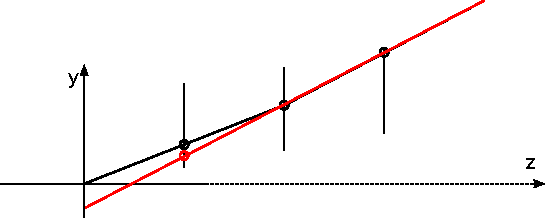
\includegraphics[width=0.6\textwidth]{vertexing/figs/isolation}
\end{center}
    \caption{Illustration of a track with a mishit.
    This view shows the Z (beam direction, beam travels left to right) and Y (magnetic field direction) axes, and three SVT layers with hits (circles).
    The true particle trajectory (black) starts at the target, is scattered at layer 2, and continues on to layer 3.
    Because the true trajectory is not straight, a better track fit can be made using a hit (red circle) from a different particle.
    The resulting track fit (red line) misses the target and, if used in a vertex fit, will lead to a best-fit vertex downstream of the target.
    }
    \label{fig:isolation_schematic}
\end{figure}

Therefore an ``isolation'' value is calculated for each of the layer 1 hits, as the distance to the closest hit in the outwards direction.
If the isolation is less than 0.5 times the track's distance of closest approach to the beamspot in the $y-z$ plane, the hit on the track may be a mishit and the closest hit might be the real hit.
If this is the case for any of the four isolations (one for each layer 1 sensor), the pair is rejected.
The effect of this cut is shown in Figure \ref{fig:isolation_performance}.

\begin{figure}[ht]
\begin{center}
    \includegraphics[width=0.6\textwidth,page=5,angle=-90]{vertexing/figs/vertcutplots}
\end{center}
    \caption{Effect of the isolation cut on events in the mass slice centered at 30 MeV, and passing all other cuts.
    By design the isolation cut has little impact on vertices with $z\approx z_{target}$, since the tracks in those pairs pass close to the beamspot.
    }
    \label{fig:isolation_performance}
\end{figure}

\subsection{Momentum Asymmetry and Positron DOCA}
Two cuts are specifically designed to reject wide-angle bremsstrahlung pairs (the layer 1 requirement also significantly reduces the rate of WABs).

Because the electron from a bremsstrahlung interaction typically carries more momentum than the photon, the electron in a WAB pair usually has higher momentum than the positron.
Heavy photons and radiative tridents have a symmetric distribution of electron and positron momentum, so a cut is used to reject pairs where the electron has much higher momentum than the positron.

If the pair conversion happens in the SVT, the positron track will curve wide of the target since the positron is roughly collinear with the photon, which does not bend in the magnetic field.
This appears in the track parameters as a positive DOCA (distance of closest approach) in the X-Z plane.
Therefore, pairs with large positive positron DOCA are rejected.

The effect of both cuts is shown in Figure \ref{fig:wabcut_performance}.

\begin{figure}[ht]
\begin{center}
    \includegraphics[width=0.35\textwidth,page=6,angle=-90]{vertexing/figs/vertcutplots}
    \includegraphics[width=0.35\textwidth,page=7,angle=-90]{vertexing/figs/vertcutplots}
\end{center}
    \caption{Effect of the WAB rejection cuts on events in the mass slice centered at 30 MeV, and passing all other cuts.
    The $z$ distributions of events rejected by these cuts are wider than the events that pass, showing that while wide-angle bremsstrahlung conversions do not have systematic shifts in vertex $z$, they contribute to the tails of the $z$ distribution.
    }
    \label{fig:wabcut_performance}
\end{figure}

\subsection{Tuning Cuts}
Data is used to tune the cuts to keep pairs with $z$ close to $z_{target}$, and reject pairs with large positive $z$.
The intent is to maximize the cut efficiency for pairs with well-reconstructed $z$, and minimize the tails of the $z$ distribution for prompt pairs (thus minimizing $z_{cut}$, and maximizing the usable signal region for heavy photons).

In general, tuning cuts on the data can introduce bias.
In this case, only the unblinded 10\% of the full dataset is being used (and will be used, even after the data is unblinded) for tuning cuts; even if a heavy photon is present in the tuning data, the number of expected events is negligible.
Also, since the cuts are not tuned for individual mass slices, any possible heavy photon signal will not be as prominent in the tuning process as it would be in the analysis.

Heavy photon Monte Carlo is used to check that none of the cuts have an unexpected adverse effect on efficiency for displaced vertices.

\clearpage
\section{Fit Inputs}

%The events passing cuts are reduced to a 2-D dataset of points $(m,z)$, where each point is the mass $m$ and vertex Z-coordinate $z$ of an event.

To test for a heavy photon at mass $m_{A'}$ and coupling $\epsilon^2$, the signal, background, and resolutions must be modeled as inputs to the analyses.

The mass cut is set to keep only events with $|m-m_{A'}|<1.4 \sigma_m(m_{A'},z)$, where $\sigma_m$ is the mass resolution expected for heavy photons with mass $m_{A'}$.
The mass resolution depends on the mass and the vertex position, and is estimated using Monte Carlo: this is explained in Section \ref{sec:mres}.
This mass window is chosen to accept a large fraction of the signal events, without accepting too many background events.
A window of $\pm1.4\sigma$ (which accepts 83.8\% of the signal events) optimizes significance for high-statistics, high-background experiments where significance is proportional to $S/\sqrt{B}$.
The optimality of this window is not exact for low statistics (where the Poisson distribution cannot be safely approximated as a Gaussian), but is still approximately true.

After cutting on $m$, the distribution of events in $z$ is studied.
An additional cut is made to keep only events with $z>z_{cut}$, rejecting the region where the background strongly dominates and there is no sensitivity to a signal.
$z_{cut}$ is chosen such that only 0.5 events are expected past $z=z_{cut}$, based on the fitted shape of the background distribution.
The amplitude of the background distribution is taken from the peak of the vertex distribution; the shape is taken from Monte Carlo as described in Section \ref{sec:tails}.

Setting limits requires knowledge of the expected signal distribution, $S(z;m_{A'},\epsilon^2)$.
This is described in Section \ref{sec:signal_shape}.

\clearpage
\subsection{Estimating the Mass Resolution}
\label{sec:mres}

The mass resolution $\sigma_m$ for a $e^+e^-$ pair depends on the momentum resolutions $\sigma_{p_{e^+}},\sigma_{p_{e^-}}$ for the two particles, the resolution $\sigma_\theta$ of the opening angle, and their covariances.
Since the opening angle and momentum measurements predominantly rely on different parts of the SVT (opening angle on the upstream half of the SVT, momentum on the downstream half), their covariance is negligible.
Neglecting the electron mass, and using the small-angle approximation for the opening angle,
\begin{equation}
m=\sqrt{(1-\cos\theta)p_{e^+}p_{e^-}} \approx \frac{1}{\sqrt{2}}\theta\sqrt{p_{e^+}p_{e^-}}
\end{equation}
\begin{equation}
\sigma_m\approx \frac{1}{\sqrt{2}}\left(\theta \frac{\sqrt{p_{e^+}p_{e^-}}}{2}\left(\frac{\sigma_{p_{e^+}}}{p_{e^+}}+\frac{\sigma_{p_{e^-}}}{p_{e^-}}\right)  + \sigma_\theta\sqrt{p_{e^+}p_{e^-}} \right)
%\sigma_m\approx \frac{1}{\sqrt{2}}(\theta\sigma_{\sqrt{p_{e^+}p_{e^-}}} + \sigma_\theta\sqrt{p_{e^+}p_{e^-}})
\end{equation}
$\theta$ is the only term in this expression with a strong dependence on $m$ or $z$: it is proportional to $m$.
Because the momentum resolution is dominated by multiple scattering, the fractional momentum resolutions $\frac{\sigma_{p_{e^+}}}{p_{e^+}}$ and $\frac{\sigma_{p_{e^-}}}{p_{e^-}}$ do not depend strongly on the momentum; nor do they depend on the track angles.
The opening angle resolution is determined by the resolutions for the two track slopes, which do not depend strongly on the track slopes, so $\sigma_\theta$ is roughly constant.
The conclusion is that $\sigma_m$ is expected to depend linearly on $m$, and not at all on $z$.

Mass resolution is measured using the Monte Carlo samples of reconstructed heavy photons described in Section \ref{sec:ap_mc}.
For each $m_{A'}$, the residual between the reconstructed mass and true mass is plotted against the true $z$.
The width of the residual distribution at each $z$ is fitted with a Gaussian to get the mass resolution at that $z$, $\sigma_m(m_{A'},z)$.
The mass resolution is fitted with a first-order polynomial in $z$:
$\sigma_m(m_{A'},z) = a_0(m_{A'}) + a_1(m_{A'}) z$.
Then the polynomial coefficients are themselves fitted with first-degree polynomials in $m_{A'}$: $a_0(m_{A'}) = a_{00} + a_{01}m_{A'}$, $a_1(m_{A'}) = a_{10} + a_{11}m_{A'}$.
The result of this procedure is a model for the mass resolution: $\sigma_m(m_{A'},z) = (a_{00} + a_{01}m_{A'}) + (a_{10} + a_{11}m_{A'}) z$.

%However $\sigma_m$ increases with $z$ as shown in Figure \ref{fig:skewed_mres}, and $a_{11}$ is significantly positive.
%This seems to be an effect of a bug in the vertex fitter, which does not correctly calculate the opening angle at the vertex.
%The reconstructed mass has a systematic dependence on the opening angle in the X-Z plane, which widens the distribution of reconstructed masses as shown in Figure \ref{fig:mass_skew}.
%If this effect is subtracted out, the mass resolution becomes constant with respect to $z$, as shown in Figure \ref{fig:fixed_mres}.

%\begin{figure}[ht]
%\begin{center}
    %\includegraphics[width=0.7\textwidth,page=4,angle=-90]{vertexing/figs/acceptance_40}
%\end{center}
    %\caption{Mass resolution vs. $z$ for 40 MeV heavy photons. The resolution gets worse with increasing $z$.}
    %\label{fig:skewed_mres}
%\end{figure}

%\begin{figure}[ht]
%\begin{center}
    %\includegraphics[width=0.7\textwidth,page=5,angle=-90]{vertexing/figs/acceptance_40}
%\end{center}
    %\caption{Mass resolution for 40 MeV heavy photons decaying near $z=30$ mm. The mass residual has a systematic dependence on the opening angle in the X-Z plane.}
    %\label{fig:mass_skew}
%\end{figure}

\begin{figure}[ht]
\begin{center}
    \includegraphics[width=0.7\textwidth,page=5,angle=-90]{vertexing/figs/acceptance_30}
\end{center}
    \caption{Mass resolution vs. $z$ for 40 MeV heavy photons in Monte Carlo.
    Top: mass residual (difference between the reconstructed mass and the true mass) vs. $z$ for 40 MeV heavy photons.
    Bottom: the widths of Gaussian fits to vertical slices of the top distribution (blue points), and a linear fit to the points (red line).
    The slope of the linear fit is consistent with 0, showing that the mass resolution is constant with respect to $z$.}
    \label{fig:fixed_mres}
\end{figure}

The fitted values of $a_{10}$ and $a_{11}$ are consistent with 0, as expected.
After this procedure, this is the mass resolution model (including statistical uncertainties in the last digits of the coefficients):
\begin{equation}
\sigma_m(m_{A'},z) = 0.00072(2) \mathrm{GeV} + 0.0382(4) m_{A'}
\end{equation}

\begin{figure}[ht]
\begin{center}
    \includegraphics[width=0.7\textwidth,page=12,angle=-90]{vertexing/figs/acceptance_data}
\end{center}
\caption{Mass resolution vs. $m_{A'}$. The blue marker is the M{\o}ller mass resolution in data.}
    \label{fig:mres_data}
\end{figure}

M{\o}ller scattering is one check of the mass resolution.
As explained in Section \ref{sec:mollers}, pairs of electrons from M{\o}ller scattering have a fixed invariant mass equal to the center-of-mass energy.
The width of the M{\o}ller mass distribution is therefore a useful check.
Figure \ref{fig:moller_mres} shows the M{\o}ller mass distribution in data, which has $\sigma_m=2.168$ MeV.
As shown in Figure \ref{fig:mres_data}, this is within 10\% of the heavy photon mass resolution from Monte Carlo (1.973 MeV).
The difference between data and Monte Carlo resolutions is believed to be due to the incomplete SVT alignment, for which work is still in progress.

\begin{figure}[ht]
\begin{center}
    \includegraphics[width=0.7\textwidth,page=18,angle=-90]{vertexing/figs/mollerplots}
\end{center}
    \caption{Distribution of reconstructed invariant mass of M{\o}ller pairs, with a Crystal Ball fit showing the mass resolution.}
    \label{fig:moller_mres}
\end{figure}

\clearpage
\subsection{Estimating the Signal Distribution}
\label{sec:signal_shape}
The expected distribution of signal events can be expressed as $\mu_{exp} s(z)$, where $\mu_{exp}$ is the expected number of reconstructed heavy photon events after the mass and $z$ cuts, and $s(z)$ is the probability density function (normalized to unit integral) of the $z$ locations.
The distribution is estimated as the following product of terms, where each term can depend on $m_{A'}$ and $\epsilon^2$:
\begin{equation}
\mu_{exp} s(z) = (N_{A'}\epsilon_{reco}(z_{target}))\frac{e^{\frac{z_{target}-z}{\gamma c \tau}}}{\gamma c \tau}\frac{\epsilon_{reco}(z)}{\epsilon_{reco}(z_{target})} \epsilon_{cut}(z)
\end{equation}
$N_{A'}$ is the number of heavy photons produced in the target.
The exponential function is the distribution of decays along $z$, and is normalized to 1.
$\epsilon_{reco}(z)$ is the efficiency to detect and reconstruct an $e^+e^-$ pair produced at a given $z$.
$\epsilon_{cut}(z)$ is the efficiency of the mass and $z$ cuts for a heavy photon with mass $m_{A'}$ decaying at a given $z$. It equals 0 for $z<z_{cut}$, and 0.838 for $z\ge z_{cut}$.

In principle, this distribution should be smeared by $\sigma_z$, the resolution of the vertex position: this is not done since the signal distribution varies slowly on the scale of $\sigma_z$ (which is 3-6 mm, depending on $m$).

\subsubsection{Production Rate and Radiative Fraction}

$N_{A'}\epsilon_{reco}(z_{target})$ is estimated using data and Equation \ref{eq:production}, which shows that $N_{A'}$ is linked to $\frac{\mathrm{d}N_{rad}}{\mathrm{d}m}$, the number of radiative tridents produced with masses around $m_{A'}$.
The data gives $\frac{\mathrm{d}N_{e^+e^-}}{\mathrm{d}m}\epsilon_{reco}(z_{target})$, the number of $e^+e^-$ pairs produced and detected in a mass window around $m_{A'}$; some fraction of these are radiative tridents.
The fraction is estimated using Monte Carlo.

The Monte Carlo samples described in Section \ref{sec:tri_mc} are used to calculate the normalized cross-sections (after detector and reconstruction efficiencies, and all cuts) for radiative tridents only, for all tridents, and for wide-angle bremsstrahlung conversions.
The radiative trident fraction is the ratio of the cross-section for radiative tridents to the total cross-section for $e^+e^-$ pairs.

\begin{figure}[ht]
\begin{center}
    \includegraphics[width=0.35\textwidth,page=5,angle=-90]{vertexing/figs/frac}
    \includegraphics[width=0.35\textwidth,page=6,angle=-90]{vertexing/figs/frac}
\end{center}
    \caption{Left: rates of processes producing $e^+e^-$ pairs, with the sum in black. Right: the radiative fraction, which is calculated by dividing the black histogram by the red histogram.}
    \label{fig:radfrac}
\end{figure}

\subsubsection{Decay Length}
The decay length is calculated using Equation \ref{eq:lifetime}, which gives the lifetime $\tau$ for a given $m_{A'}$ and $\epsilon^2$.
The boost $\gamma$ equals $E_{beam}/m_{A'}$ if the heavy photon takes the full beam energy, but this is not completely accurate; in reality the average boost is slightly less than the maximum.

Monte Carlo samples are used to find the correct distribution of decay lengths.
As shown in Figure \ref{fig:decay_z_truth}, the decay $z$ is plotted for an MC sample of heavy photons with mass $m_{A'}$ and an arbitrary lifetime, with the requirement that the heavy photon momentum be at least $0.8E_{beam}$ (matching the analysis cut), and fit with an exponential.
The decay constant of the exponential is compared to the $\gamma c \tau$ that would be expected from $\gamma=E_{beam}/m_{A'}$; this shows that the typical $\gamma$ is roughly $0.95E_{beam}/m_{A'}$.

\begin{figure}[ht]
\begin{center}
    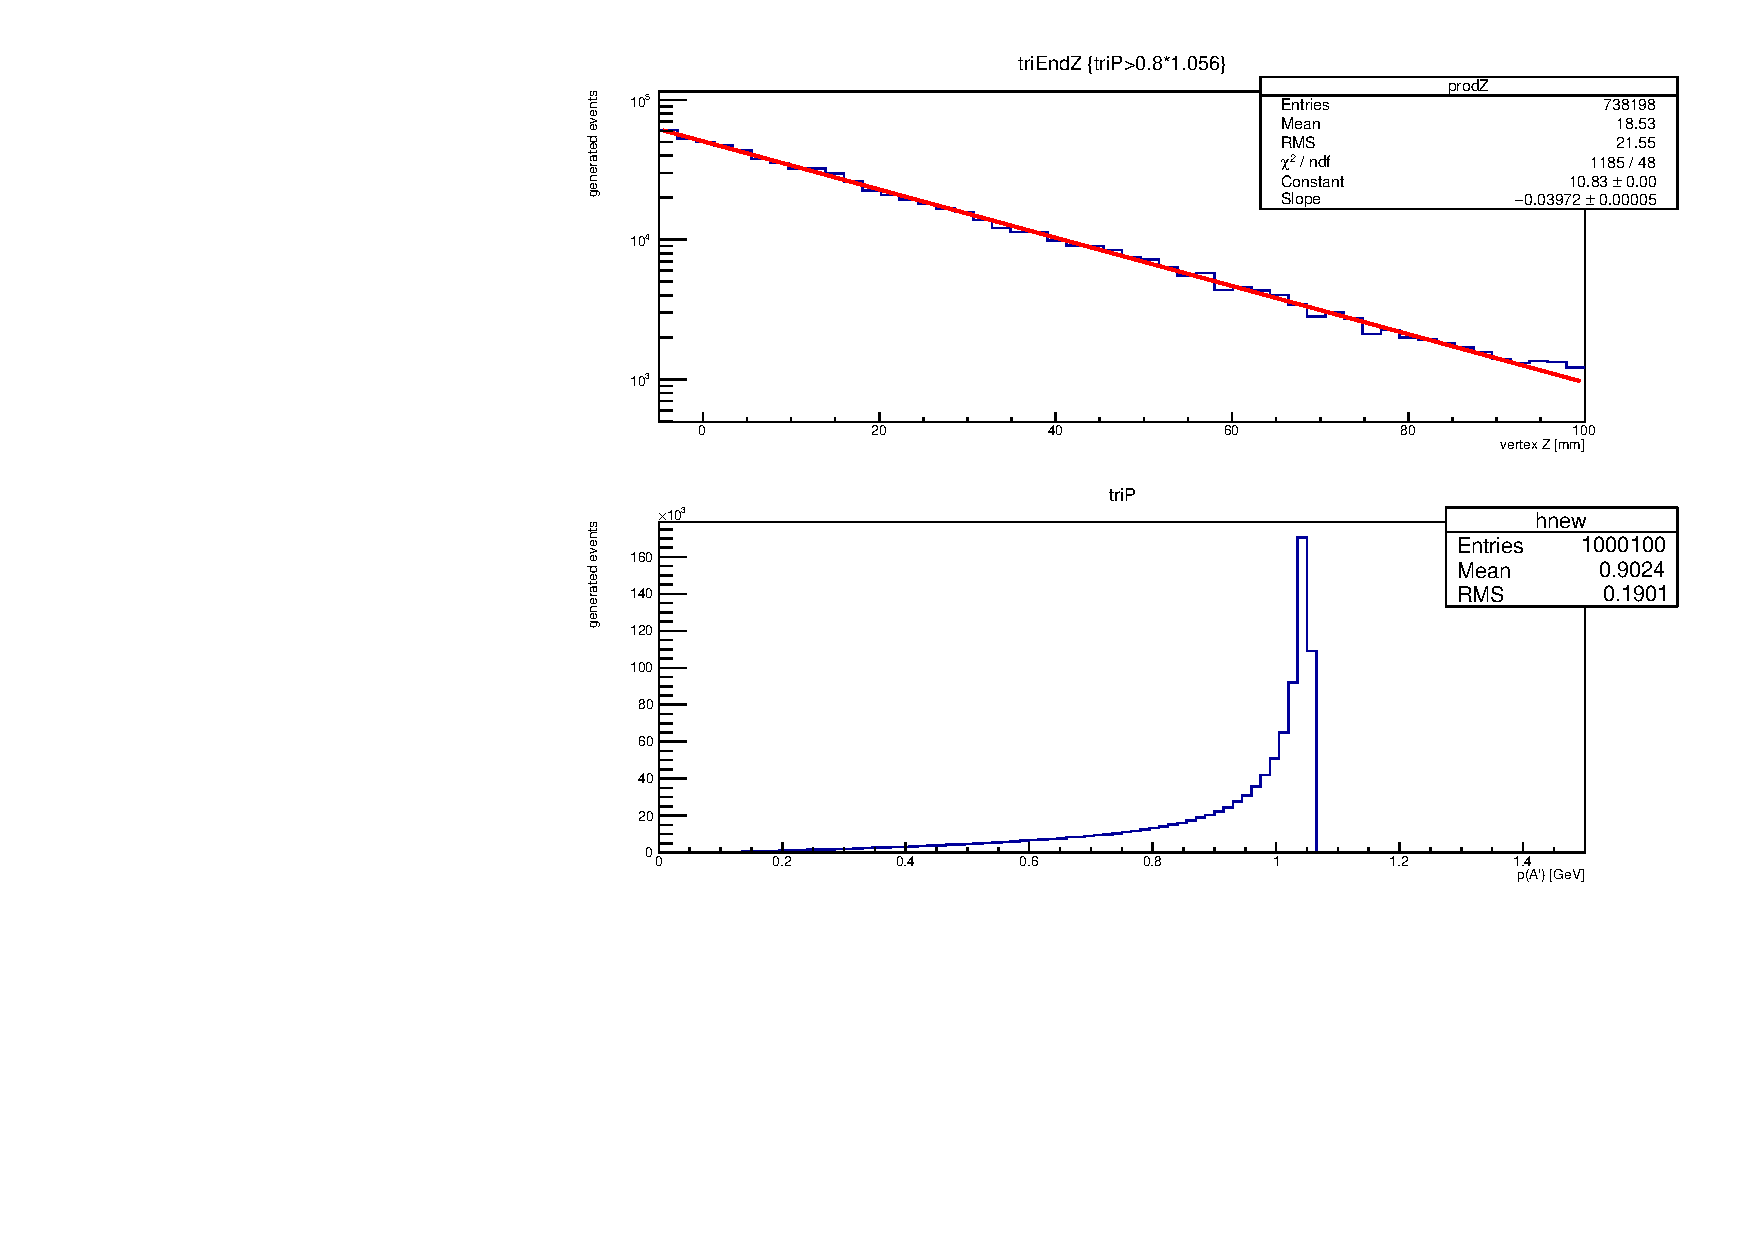
\includegraphics[width=0.7\textwidth,page=1,angle=-90]{vertexing/figs/acceptance_40}
\end{center}
    \caption{Top: distribution of decay $z$ for heavy photons ($m_{A'}=40$ MeV, $c\tau=1$ mm) carrying at least 80\% of the beam momentum. Bottom: the momentum distribution for the heavy photons.}
    \label{fig:decay_z_truth}
\end{figure}

\subsubsection{Efficiency}
\label{sec:efficiency_z}

The efficiency $\epsilon_{reco}$ for reconstructing a heavy photon decay depends on $m_{A'}$ and the decay $z$.
The measurement of the radiative trident rate implicitly includes a factor of $\epsilon_{reco}(m_{A'},z_{target})$, so Monte Carlo is only needed to estimate $\frac{\epsilon_{reco}(m_{A'},z)}{\epsilon_{reco}(m_{A'},z_{target})}$, the efficiency falloff as a function of vertex displacement.
This assumes that any detector-based inefficiencies not represented in the Monte Carlo are independent of $z$.

The efficiency falls off with $z$ because the further downstream the decay, the larger the opening angle in the Y-Z plane necessary to hit layer 1 of the SVT.
At some cutoff value of $z$ it is no longer possible for both the electron and the positron to hit layer 1; the efficiency starts to fall off well before that cutoff.
This effect is more severe for lower $m_{A'}$, where the opening angle is smaller.

The efficiency is measured using the Monte Carlo samples of generated and reconstructed heavy photons described in Section \ref{sec:ap_mc}.
For each $m_{A'}$, the distribution of decay $z$ is filled both for generated and reconstructed heavy photons (examples in the top halves of Figures \ref{fig:decay_z_truth} and \ref{fig:eff_z} respectively).
The ratio of the two distributions gives $\epsilon_{reco}(m_{A'},z)$; for $m_{A'}=40$ MeV, this is shown in the bottom of Figure \ref{fig:eff_z}.
This is scaled so it equals 1 at $z=z_{target}$, and is fitted with a function of the form $\frac{\epsilon_{reco}(m_{A'},z)}{\epsilon_{reco}(m_{A'},z_{target})} \approx \exp(p_3 z^3 + p_2 z^2 + p_1 z + p_0)$.
The parameters $p_3$, $p_2$, $p_1$, and $p_0$ are fit with polynomials in $m_{A'}$: $p_0$ and $p_1$ are fit with first-order polynomials, and $p_2$ and $p_3$ are fit with third-order polynomials.

\begin{figure}[ht]
\begin{center}
    \includegraphics[width=0.7\textwidth,page=2,angle=-90]{vertexing/figs/acceptance_40}
\end{center}
    \caption{Top: distribution of decay $z$ for reconstructed heavy photons ($m_{A'}=40$ MeV, $c\tau=1$ mm) after all cuts. Bottom: efficiency curve $\frac{\epsilon_{reco}(m_{A'},z)}{\epsilon_{reco}(m_{A'},z_{target})}$, with fit.}
    \label{fig:eff_z}
\end{figure}

\clearpage
\subsection{Fitting the Background Distribution}
\label{sec:tails}
The background distribution consists of a Gaussian core and a non-Gaussian tail.
The width of the Gaussian core is set by multiple scattering and is well understood, but the tails extend much farther than the Gaussian.
For $z>z_{cut}$, the background distribution is dominated by the tails: $z_{cut}$ is typically at least $5\sigma_z$.

The background distribution is estimated from Monte Carlo.
This is necessary because if the background distribution were fit from the data, and there is actually a heavy photon signal in the data, the fit would be pulled so as to understate the size of the signal.
As in Figure \ref{fig:vertex_data-mc}, comparisons of the background distribution in Monte Carlo and data show that the Monte Carlo accurately simulates the processes that control the vertex resolution: the resolution in the Gaussian core and tails found in Monte Carlo are good fits to the data.

\begin{figure}[ht]
\begin{center}
    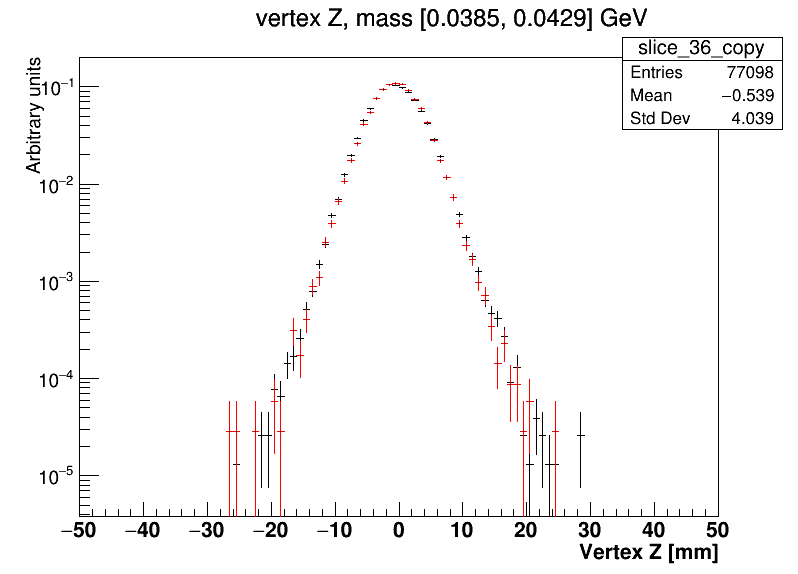
\includegraphics[width=0.7\textwidth]{vertexing/figs/slice-36}
\end{center}
\caption{Comparison of vertex Z distributions between data (black) and Monte Carlo (red).}
    \label{fig:vertex_data-mc}
\end{figure}

The 2-dimensional vertex distribution from Monte Carlo is scanned in $m$, using the same mass cut that is used for the analysis.

The background distribution is fit with a 4-parameter piecewise function defined from a Gaussian and an exponential.
The Gaussian is defined with the usual parameters of mean $\bar{z}$ and standard deviation $\sigma$.
The parameter $b$ defines the distance from the Gaussian's mean where the distribution transitions to the exponential.
The exponential is defined in terms of a tail length $l$, and its amplitude is fixed by the requirement that the function be continuous.
This function is similar to the ``GaussExp'' function described in \cite{cms_collaboration_search_2015}, except GaussExp fixes the exponential's decay length by requiring that the function be continuously differentiable.
\begin{equation}
B(z;\bar{z},\sigma,b,l)=
\begin{cases}
e^{-\frac{(z-\bar{z})^2}{2\sigma^2}} &\text{if } z\le\bar{z}+b,\\
e^{-\frac{b^2}{2\sigma^2} - (z-\bar{z}-b)/l}  &\text{if } z\ge\bar{z}+b
\end{cases}
\label{eq:gaussexp}
\end{equation}

The values of $b$ and $l$ found at each $m_{A'}$ are fitted to cubic polynomials in $m_{A'}$.
When estimating $B(z)$ for data, the values of $b$ and $l$ are fixed to the values found for Monte Carlo, but the Gaussian parameters are allowed to float.

As shown in Figure \ref{fig:vz_1d} for a representative mass slice, this procedure fits the data well for several orders of magnitude.
However, it is not immediately obvious whether the background model completely describes the extreme tail of the distribution.

\subsubsection{Characterizing Excess Backgrounds}
\label{sec:excess_background}
If the tails of the vertex distribution were completely described by the exponential tail of the background model of Equation \ref{eq:gaussexp}, each mass slice should by construction (on average, and in the absence of a possible heavy photon signal) contain 0.5 events with $z>z_{cut}$.
But as seen in Figure \ref{fig:n_candidates}, most mass slices contain more than one event with $z>z_{cut}$, and some contain as many as 4 events; this is a significant excess.
This indicates either that there is a heavy photon in the data, or that there is a background not described by the background model.

\begin{figure}[ht]
\begin{center}
    \includegraphics[width=0.7\textwidth,page=8,angle=-90]{vertexing/figs/golden_mres_output}
\end{center}
\caption{Number of events found with $z>z_{cut}$ in each mass slice, as a function of the center mass of the mass slice.
Since mass slices overlap, a single event appears many times in this plot.
If the background model fully describes the data, the mean number per mass slice of events with $z>z_{cut}$ should be 0.5.}
    \label{fig:n_candidates}
\end{figure}

\begin{figure}[ht]
\begin{center}
    \includegraphics[width=0.7\textwidth,page=4,angle=-90]{vertexing/figs/golden_mres_output}
\end{center}
\caption{The set of events that appear with $z>z_{cut}$ in at least one mass slice.
This is the same histogram as Figure \ref{fig:zvsmass}, but only plotting events above $z=z_{cut}$ (the black curve).
Some events are close to $z=z_{cut}$, but some events are substantially above the black line ($z\gg z_{cut}$).}
    \label{fig:zvsmass_candidates}
\end{figure}

The events with $z>z_{cut}$ can be characterized by their distributions in $z$ and in mass.
Events consistent with the background model should have $z$ close to $z_{cut}$ (the median $z-z_{cut}$ is proportional to $l$), but be uniformly distributed in mass, with an average of 0.5 events per mass slice.
Any other component of the background might have a different distribution in $z$, but will be broadly distributed in mass.
Events from heavy photon decays should have large $z$ and a tight distribution in mass (limited by the mass resolution).

If the excess events are described by the background model, the events with $z>z_{cut}$ in a mass slice should be distributed according to the exponential distribution.
Transforming by the cumulative distribution function (CDF) of the exponential, $z\to 1-e^{(z_{cut}-z)/l}$, gives the quantile of each event in the background model; if the background model describes the events, the quantiles should be distributed uniformly.
Figure \ref{fig:candidates_rescaled} shows the quantile histogram for one mass slice; Figure \ref{fig:zvsmass_candidates_rescaled} shows the quantiles for all mass slices.
Some of the events with $z>z_{cut}$ do appear to follow this pattern, but some have large quantiles, meaning that they have $z$ larger than would be typical from sampling the background model.

\begin{figure}[ht]
\begin{center}
    \includegraphics[width=0.6\textwidth,page=60,angle=-90]{vertexing/figs/golden_mres}
\end{center}
\caption{The background CDF values (quantiles) for events in the mass slice centered at $m_{A'}=35.6$ MeV that have $z>z_{cut}$ (this is the same mass slice as Figure \ref{fig:vz_1d}).
The two events with $z\approx 35$ have quantiles close to 1, suggesting that their values of $z$ are larger than would be expected from the background model.}
    \label{fig:candidates_rescaled}
\end{figure}

\begin{figure}[ht]
\begin{center}
    \includegraphics[width=0.7\textwidth,page=7,angle=-90]{vertexing/figs/golden_mres_output}
\end{center}
\caption{The background quantiles for events that have $z>z_{cut}$ in each mass slice.
This is not a true histogram; each vertical column is a histogram similar to Figure \ref{fig:candidates_rescaled}, but a given event is plotted in every mass slice where it appears.
The quantile for a given event changes with the mass slice because $z_{cut}$ depends on the mass slice.
}
    \label{fig:zvsmass_candidates_rescaled}
\end{figure}

If we (somewhat arbitrarily) separate the two sets of events by cutting at a quantile of 0.9, the events with low quantiles contribute 0.52 events per mass slice; this suggests that these events are consistent with the background model and occur with the correct frequency, but the high-$z$ events with quantiles above 0.9 are in excess of the expected background.
These are the five events on the upper right of Figure \ref{fig:zvsmass_candidates}, with masses between 30 and 50 MeV and $z>30$ mm.

The five events isolated by the quantile cut are spread broadly in mass.
As a group, their RMS in mass is 4.2 MeV, much larger than the estimated mass resolution (2.2 MeV) at the mean mass (38.2 MeV).
No mass slice captures more than three of these events; if all five events had the same true mass, the lowest- and highest-mass events would be deviations of more than $2\sigma_m$.
In other words, it is unlikely that these events originate from a process with a fixed mass.
These events do not match the signature of a heavy photon.

The rate of these events is also not consistent with a heavy photon, or with beam-gas interactions.
The expected number of heavy photon decays in this data is much less than 1, as discussed in \ref{sec:results}.
Beam-gas interactions, where beam electrons interact with residual gas in the beamline to create $e^+e^-$ pairs downstream of the target, are another potential source of displaced vertices, but cannot explain these events.
The beamline vacuum was measured to be in the $10^{-5}$ torr range, which would (under generous assumptions) contribute less than 0.01 event to this data set.

There is other evidence that these events are a rare detector background and not a heavy photon.
A sample of trident Monte Carlo (with 1/3 as much integrated luminosity as the data used for this analysis) contains one similar event: see Figure \ref{fig:zvsmass_candidates_mc}.
This suggests that these events are a background that can be reproduced and understood in Monte Carlo.

Since the current rate of the excess background is greater than the expected rate of heavy photon decays, rejecting them is essential to the full HPS analysis: the number of excess background events will scale with luminosity, and will always overpower any heavy photon signal.
The current vertex cuts have mostly been tuned to reject the exponential tail of the vertex $z$ distribution, or to reject specific detector backgrounds.
Studying the excess background in Monte Carlo is likely to identify a specific process that produces these events, and may lead to a specific cut that can reject them.

\begin{figure}[ht]
\begin{center}
    \includegraphics[width=0.7\textwidth,page=4,angle=-90]{vertexing/figs/mc_mres_output}
\end{center}
\caption{The set of events that appear with $z>z_{cut}$ in at least one mass slice (similar to Figure \ref{fig:zvsmass_candidates}), for a trident Monte Carlo sample.
One event has $z\gg z_{cut}$.
}
    \label{fig:zvsmass_candidates_mc}
\end{figure}

\clearpage
\section{Finding Signal Significance}
\label{sec:significance}
The signal significance is a measure of the inconsistency of the data with the background-only assumption.
It is expressed in terms of a $p$-value, which is the probability under the background-only hypothesis of observing an apparent signal that is at least as significant as what was seen in the data.
The convention in particle physics is to convert the $p$-value to an equivalent significance $Z$, defined such that $p$ equals the $p$-value of a $Z$-sigma upward fluctuation in a Gaussian variable.

For this analysis, the significance at a given $m_{A'}$ is calculated using $n$, the number of pairs in the mass slice with $z>z_{cut}$, and $b$, the number of background events expected.
$p$ equals the probability $P(n;b) = \sum^{\infty}_{k=n} \frac{b^k}{k!} e^{-b}$ of drawing at least $n$ events from a Poisson distribution with mean $b$.
%However, a value of $P(n;b)>0.5$ indicates that the observed number of events is small relative to the expected background.
%In this case a downward statistical fluctuation is assumed, and the data is considered consistent with the background-only assumption: in this case $p=0.5$, since under the background-only assumption downward fluctuations happen half the time.

According to the expected background distribution and the definition of $z_{cut}$, $b$ should equal 0.5.
However, as shown in Figure \ref{fig:n_candidates} and explained in \ref{sec:excess_background}, there appears to be an additional background that is above the 0.5 level, and varies smoothly with $m$.
Because this cannot be a heavy photon, we can treat it as part of the background.

Since the background is larger than 0.5, $b$ must be approximated using the data.
$b$ for a given $m_{A'}$ hypothesis must be approximated in a way that is not biased by the data in the $m_{A'}$ mass slice.
This is done for every mass slice as shown in Figure \ref{fig:bkg_fit} by taking the mass slices that do not overlap with the $m_{A'}$ mass slice, and fitting the trend in $n$ as a quadratic function of $m_{A'}$.
Assuming there is only one heavy photon, this procedure yields an estimate of $b$ for a $m_{A'}$ hypothesis that is not perturbed by the possible presence of a heavy photon.

\begin{figure}[ht]
\begin{center}
    \includegraphics[width=0.7\textwidth,page=164,angle=-90]{vertexing/figs/golden_mres}
\end{center}
\caption{Unbiased fit to estimate the background rate past $z_{cut}$ in the mass slice centered at 35 MeV.}
    \label{fig:bkg_fit}
\end{figure}

The $p$-values from this procedure are shown in Figure \ref{fig:pval}.
The smallest $p$-value is 0.0661, but it is not correct to use this as the significance of the data set.
These are ``local'' $p$-values: the $p$-value for a mass slice represents the consistency of that slice of the data with the background-only hypothesis.
But the objective of this analysis is to find the significance of the full data set, not individual slices: how consistent is the data with the background-only hypothesis?
This is expressed by a ``global'' $p$-value.
\begin{figure}[ht]
\begin{center}
    \includegraphics[width=0.7\textwidth,page=12,angle=-90]{vertexing/figs/golden_mres_output}
\end{center}
\caption{Local $p$-value for finding the observed number of events at each $m_{A'}$. The minimum value is 0.0661.}
    \label{fig:pval}
\end{figure}


The ``global'' $p$-value is found by taking the minimum of all local $p$-values, and finding the probability of finding a $p$-value at least as significant as this one.
The global $p$-value is always larger (less significant) than the local $p$-value because there are multiple local $p$-values.
This is known as the ``look-elsewhere effect.''

A simple brute-force method of finding the global $p$-value is to run a Monte Carlo simulation of the background-only hypothesis and tabulate the probability of finding a given minimum local $p$-value.
The cumulative distribution of minimum local $p$-values, scaled to 1, gives the mapping to global $p$-value.

The Monte Carlo model of the background-only hypothesis must reflect the background seen in the data.
The distribution of events past $z_{cut}$ is fit to a quadratic function, and data sets are drawn from this distribution: there are 12 events past $z_{cut}$, and so the number of events in each Monte Carlo data set is drawn from a Poisson distribution with a mean of 12.
The distribution of minimum local $p$-values is shown on the left side of Figure \ref{fig:trials}, and the cumulative distribution is on the right.

\begin{figure}[ht]
\begin{center}
    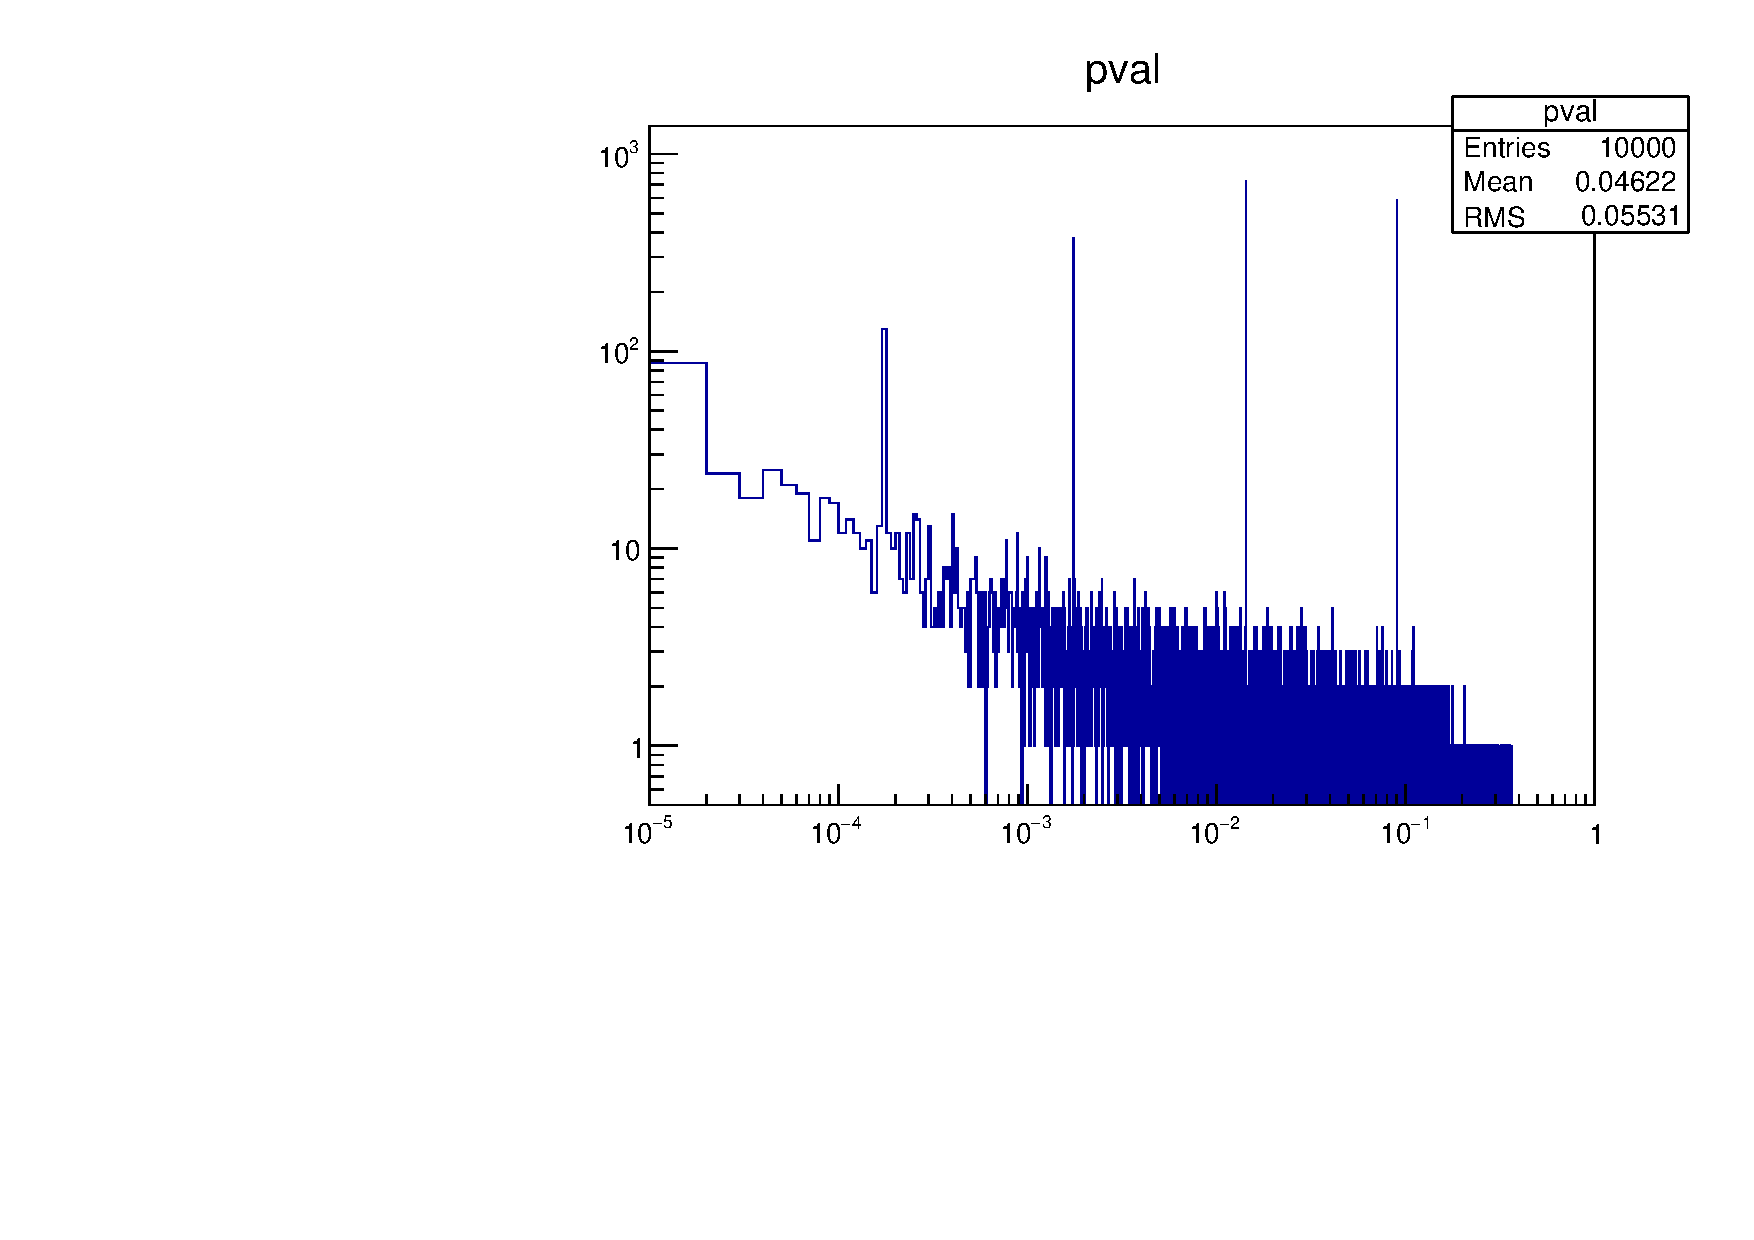
\includegraphics[width=0.35\textwidth,page=1,angle=-90]{vertexing/figs/trials}
    \includegraphics[width=0.35\textwidth,page=6,angle=-90]{vertexing/figs/trials}
\end{center}
\caption{Left: distribution of the most significant $p$-values from 10000 runs of toy Monte Carlo. Right: mapping from local to global $p$-values.}
    \label{fig:trials}
\end{figure}

After this procedure, the global $p$-value is found to be 0.72 for a local $p$-value of 0.0661.
This is completely consistent with the background-only hypothesis; it means that in fact the local $p$-value is slightly less significant than the median $p$-value.
Expressed as a equivalent one-sided significance for a Gaussian, the significance of this result is $-0.59\sigma$.

\clearpage
\section{Setting Limits}
\label{sec:limits}
An upper limit on the heavy photon production at a given $m_{A'}$ and $\epsilon^2$ is the maximum rate at which heavy photons could be produced, and still be consistent with the data.
The confidence level used for this analysis is 90\%: in other words, if a heavy photon signal does exist at a given rate, the limit set by this analysis will (incorrectly) exclude that signal rate only 10\% of the time.
The meaningful target for this analysis is the heavy photon production rate given by Equation \ref{eq:production}; if the upper limit at a given $m_{A'}$ and $\epsilon^2$ is below that rate, the analysis has (at 90\% CL) excluded the possibility of a heavy photon at that $m_{A'}$ and $\epsilon^2$.

Upper limits do not distinguish between a lack of sensitivity (insufficient data to say anything meaningful about the presence or absence of a signal) and the presence of a signal: the upper limit will be high in either case.

\subsection{Optimum Interval Method}
The method chosen for setting limits is the ``optimum interval'' method by Yellin \cite{yellin_finding_2002}.
This method was developed for dark matter direct detection experiments, and is intended for experiments where the signal shape is known, but the backgrounds are not fully understood and there is the possibility of an unexpected background.
A particular strength of the method is that it minimizes the influence of a background that is concentrated in one part of the data distribution.
This analysis uses Yellin's implementation of the optimum interval method, which is publicly available \cite{yellin_optimum_2011}.

The optimum interval method sets a one-sided upper limit (with confidence level $C$) on the number of signal events $\mu$ in a one-dimensional data set, where the shape of the signal distribution is known.
For HPS, the data set is the distribution of vertex $z$ locations, after applying the mass and $z_{cut}$ cuts; the signal distribution is the $s(z)$ found in Section \ref{sec:signal_shape} for the $m_{A'}$ and $\epsilon^2$ being tested.

The method works by testing a proposed signal rate $\mu$ against the data with a confidence level $C$.
The cumulative distribution function of the signal, $S(z)$, is known.
A change of variables is made from the measured variable $z$ to a new variable $x=\mu S(z)$.
Under the signal assumption, the expected distribution of the data is uniform in $x$ with unit density, and has total width $\mu$.
An interval $(x_1,x_2)$, with $x_1, x_2 \in [0,\mu]$, contains a number of expected signal events equal to its width $\Delta x = x_2-x_1$.
If an unexpected background is present and is distributed differently from the signal, the data will not be distributed uniformly in $x$, and events will be spaced more widely where the background is not present.

The next step is to search for the ``optimum interval,'' the interval that most strongly rejects the proposed signal rate.
This is the interval $(x_1,x_2)$ that contains the smallest number of actual events $n$ relative to its width $\Delta x$.
Put another way, if the function $C_n(\Delta x,\mu)$ is the probability that all intervals of width $\Delta x$ contain more than $n$ events, the optimum interval is the $(x_1,x_2)$ that maximizes $C_n(\Delta x,\mu)$.

For the optimum interval, $x_1$ and $x_2$ always coincide with 0, $\mu$, or events in the data (otherwise the interval can be widened to increase $\Delta x$ without changing $n$).
Thus the program only needs to loop over every interval between two events, of width $x$ expected events and containing $n$ actual events.
The value of $C_n(\Delta x,\mu)$ for the optimum interval is called $C_{Max}$, and if it exceeds a threshold $\bar{C}_{Max}(C,\mu)$, $\mu$ is rejected with confidence level $C$.
The upper limit on $\mu$ is the value for which $C_{Max}=\bar{C}_{Max}(C,\mu)$.

%The function $C_n(x,\mu)$ is the probability that all intervals containing $n$ events are narrower than this one (that is, that no interval with $n$ events has this low a ratio of actual to expected events).
%The interval with largest value of $C_n(x,\mu)$ is the ``optimum interval'' that most strongly rejects the proposed signal rate.
%The largest value found is called $C_{Max}$, and if it exceeds a threshold $\bar{C}_{Max}(C,\mu)$, $\mu$ is rejected with confidence level $C$.
%The upper limit on $\mu$ is the value for which $C_{Max}=\bar{C}_{Max}(C,\mu)$.

The functions $C_n(x,\mu)$ and $\bar{C}_{Max}(C,\mu)$ pay the statistical penalties for using the data to pick the best interval.
Since they are not specific to the signal distribution, they are calculated using Monte Carlo and stored in lookup tables that are distributed with the software.

The optimum interval method can be used with a known background; in this case, the known background density is added to the signal density.
Since the known background for HPS falls off rapidly, relatively little is to be gained from this: after the cut in $z$, the remaining known background is tightly clustered at the edge of the range of $z$, so the optimum interval method effectively ignores it even without subtraction.
Therefore the known background is not used as an input to the optimum interval calculation.

A toy model was used to assess the optimum interval method for use in HPS, and the results are shown in Figure \ref{fig:optimum_interval_demo}.
The toy signal and background are both exponential distributions, but the background has a short decay length of 2, and the signal has a long decay length of 20; in units of mm, these are typical values for HPS.
10000 background events are generated; there is no signal.
A nuisance background of 100 events, with a decay length of 10, is present in the plot on the right.
The different limits (as a number of signal events) are plotted as a function of $z_{cut}$

The optimum interval method was compared against cut-and-count limits using the Feldman-Cousins method \cite{feldman_unified_1998}.
Both methods were run with and without subtracting the known background.
As expected, the upper limits from the optimum interval method are always as strong as, or stronger than, the upper limits from the cut-and-count method given the same information.

Optimum interval limits are insensitive to background events at the edge of the search range.
This can be seen around $z=22$ and $z=26$ in the right-hand plot, where there are events from the nuisance background: the cut-and-count limits jump up discontinuously when $z_{cut}$ moves past the event, but the optimum interval limits vary smoothly.
It is still clear that it makes sense to avoid as much background as possible, so setting $z_{cut}$ for expected 0.5 background events is still appropriate.

The optimum interval method can be used with or without subtracting a known background.
This test shows that the performance is not dramatically better when subtracting the known background.

\begin{figure}[ht]
\begin{center}
    \includegraphics[width=0.35\textwidth,page=6,angle=-90]{vertexing/figs/toy_nothing}
    \includegraphics[width=0.35\textwidth,page=6,angle=-90]{vertexing/figs/toy_nosignal}
\end{center}
    \caption{Comparison of the optimum interval method with cut-and-count using Feldman-Cousins limits. The y-axis is the limit on the total signal rate as a fraction of the background rate. 
        The background (10000 events) has decay length 2, the signal has decay length 20, and the unexpected background (100 events) has decay length 5. Left plot is with only the expected background (no signal); right plot is with the unexpected background added (still no signal). The $z_{cut}$ for 0.5 expected background events is 19.8.}
    \label{fig:optimum_interval_demo}
\end{figure}

\subsection{Results}
\label{sec:results}
The optimum interval method gives limits at 90\% confidence level on $\mu$, the number of signal events past $z_{cut}$ and after acceptance and efficiency effects.
Dividing the limit on $\mu$ by $\mu_{exp}$, the expected number of signal events for a heavy photon, gives a limit on the dimensionless ratio of the true production rate to the expected production rate for a heavy photon.
A limit on $\mu/\mu_{exp}$ of 1 or less means the heavy photon is excluded (at 90\% CL) at that $m_{A'}$ and $\epsilon^2$.

The value $\mu_{exp}$ is itself of some interest: it relates directly to the strongest possible limit (obtained for the case where no events are observed in the mass slice with $z>z_{cut}$).
An exclusion at 90\% CL is only possible if $\mu_{exp}>2.303$; this is true not only for the optimal interval method but in general, since if $\mu_{exp}<2.303$ there is at least a 10\% probability of seeing no signal events even if a heavy photon exists.
%Conversely, if $\mu_{exp}>2.303$ the optimum interval method will find an exclusion as long as there are no background events in the signal box, or the background events in the signal box are clustered near $z_{cut}$.

The limits from this analysis are shown in Figure \ref{fig:upper_limit}, which shows that this analysis, on this data, is a factor of 115 from excluding any portion of the parameter space.
As shown in Figure \ref{fig:detectable}, $\mu_{exp}$ 0.032 at most, which is too small for exclusion even in the absence of excess background events.

\begin{figure}[ht]
\begin{center}
    \includegraphics[width=0.7\textwidth,page=15,angle=-90]{vertexing/figs/golden_mres_output}
\end{center}
\caption{90\% CL upper limit on $\mu/\mu_{exp}$, the ratio of the true production rate to the expected production rate for a heavy photon. A value of 1 would mean exclusion; the lowest contour on this plot is 200, and the lowest point (at $m_{A'}=49$ MeV, $\epsilon^2=2.1\times 10^{-9}$) is 115.
    The vertical ridges in this plot correspond to the locations of events in mass space.}
    \label{fig:upper_limit}
\end{figure}

\begin{figure}[ht]
\begin{center}
    \includegraphics[width=0.7\textwidth,page=16,angle=-90]{vertexing/figs/golden_mres_output}
\end{center}
    \caption{$\mu_{exp}$, the number of detectable heavy photon events expected with $z>z_{cut}$. The highest contour is at 0.03 events, and the highest point is 0.032.}
    \label{fig:detectable}
\end{figure}

\subsubsection{Reach Projections for the 2015 Run}
\label{sec:reach_projections}
Several factors will improve this reach in future iterations of this analysis.
First, the number of events with $z>z_{cut}$ was larger than predicted by the background fit.
Better background rejection cuts may be able to reduce this background, and bring the reach closer to the bound set by $\mu_{exp}$.
The reach with zero events with $z>z_{cut}$ is shown in Figure \ref{fig:upper_limit_nosignal}, where the strongest predicted limit is down to 86.2.
If, after refining cuts, the background shape comes to match the exponential form used in this analysis, the reach will be very close to this zero-events reach.

\begin{figure}[ht]
\begin{center}
    \includegraphics[width=0.7\textwidth,page=15,angle=-90]{vertexing/figs/golden_mres_nosignal_output}
\end{center}
\caption{Predicted 90\% CL upper limit on $\mu/\mu_{exp}$, assuming no events with $z>z_{cut}$. A value of 1 would mean exclusion; the lowest contour on this plot is 90, and the lowest point is 86.2.}
    \label{fig:upper_limit_nosignal}
\end{figure}

Second, this analysis only used the unblinded fraction of the 2015 data.
The full set increases integrated luminosity by a factor of 9.77 (from 199 to 1166 nb$^{-1}$), and therefore the number of detectable heavy photons.
Since $z_{cut}$ must be increased to keep the level of background at 0.5 events per mass slice, $\mu_{exp}$ does not scale linearly with the amount of data.
As shown in Figure \ref{fig:upper_limit_fullset}, this improves the exclusion to 14.7.

\begin{figure}[ht]
\begin{center}
    \includegraphics[width=0.7\textwidth,page=15,angle=-90]{vertexing/figs/golden_fullset_mres_nosignal_output}
\end{center}
\caption{Predicted 90\% CL upper limit on $\mu/\mu_{exp}$, projected for the full 2015 data set, and assuming no events with $z>z_{cut}$. A value of 1 would mean exclusion; the lowest contour on this plot is 20, and the lowest point is 14.7.}
    \label{fig:upper_limit_fullset}
\end{figure}

Finally, this analysis only used the events where both tracks made hits in layer 1 of the SVT.
As explained in Section \ref{sec:layer1_cut}
Figure \ref{fig:eff_z_alllayers} shows the difference in efficiency between the current analysis and the full acceptance.
Doing this will require tuning cuts separately for the sets of events that miss layer 1, and combining the data sets (the optimum interval method can be used for this \cite{yellin_ways_2011}).
As shown in Figure \ref{fig:upper_limit_fullset_alllayers}, this improves the exclusion to 6.68.
The mass range of the search is also substantially improved, because the lower values of $m_{A'}$ are more strongly affected by the layer 1 requirement.

%\begin{table}[ht]
    %\begin{center}
        %\caption{Assumptions used for the 2015 reach estimate.}
        %\begin{tabular}{lp{0.5\textwidth}}
            %\hline \hline
            %Beam energy & 1.056 GeV \\
            %Integrated luminosity & 1166 nb$^{-1}$ (equivalent to 50 nA, 1.69 days, target thickness 0.116\% $X_0$) \\
            %Efficiency dependence on $z$ & From Monte Carlo, with no layer 1 requirement \\
            %Efficiency at $z_{target}$ & From Monte Carlo \\
            %\hline \hline
        %\end{tabular}
        %\label{tab:reach_assumptions} 
    %\end{center}
%\end{table}

\begin{figure}[ht]
\begin{center}
    \includegraphics[width=0.7\textwidth,page=15,angle=-90]{vertexing/figs/golden_fullset_mres_allayers_nosignal_output}
\end{center}
\caption{Predicted 90\% CL upper limit on $\mu/\mu_{exp}$, projected for the full 2015 data set, using the full HPS acceptance, and assuming no events with $z>z_{cut}$. A value of 1 would mean exclusion; the lowest contour on this plot is 7, and the lowest point is 6.68.}
    \label{fig:upper_limit_fullset_alllayers}
\end{figure}

Some data was taken in 2015 with the SVT opened wider than its nominal position (silicon at 1.5 mm from the beam, instead of 0.5 mm).
The integrated luminosity is similar to the data that was used in this analysis, but the acceptance is worse.
At best, this can only double $\mu_{exp}$, so even using this data there will be no excluded region.

Reach projections for the 2016 data and the planned 2018 run are in progress.

\subsubsection{Reach Comparison with 2014 Proposal}
\label{sec:proposal_reach}
The reach estimates in the 2014 proposal (see Figure \ref{fig:reach}) are substantially different from the projected reach shown above.
The proposal estimates were made assuming 1 week of beam time, and used some assumptions that are now understood to be inaccurate.
In addition, the trident rates in data are different from the rates in Monte Carlo trident samples.
Even accounting for these differences, there are significant differences between the $\mu_{exp}$ estimated using this analysis, and the $\mu_{exp}$ that was used for reach estimates in the proposal.

The reach estimates for the proposal were made by calculating $\mu_{exp}$ assuming the same procedure presented here: apply cuts to reduce the backgrounds at large $z$, make a resolution-limited mass slice and apply a $z_{cut}$ that reduces the background to 0.5 expected events.

%The exclusion region in $(m_{A'},\epsilon^2)$ space was defined as the region with $\mu_{exp}>2.4$ events.
%This was intended as a $2\sigma$ confidence level exclusion, based on the probability of observing 0 events given a background rate of 0.5 events and a signal rate of 2.4 events.
%This reasoning overestimates the exclusion region for a given confidence level, since it assumes that the exclusion region is found by a cut-and-count analysis that excludes parts of parameter space where $\mu_{exp}>2.4$ and 0 events were observed; there will be no exclusion in mass slices where background events are observed.

These are assumptions that were made for the proposal, and how each differs from our current understanding of the experiment:
\begin{itemize}
\item The integrated luminosity was expected to be 1 week of 50 nA beam, on a target with the nominal thickness of 0.125\% of a radiation length; the actual target was somewhat thinner, at 0.116\% $X_0$.
\item The beam energy was expected to be 1.1 GeV; in reality it was 1.056 GeV. The beam energy affects the vertex resolution, mass scale and production rates, but the difference in beam energy is small.
\item Efficiency for heavy photons was assumed to be uniform to $z=100$ ($\epsilon_{reco}(m_{A'},z) = \epsilon_{reco}(m_{A'},z_{target})$).
This is of course not true, as explained in Section \ref{sec:efficiency_z}.
The impact depends on mass (just like the efficiency) but is roughly a factor of 2 to 3.
\item Rates for heavy photons and trident backgrounds were estimated using a MadGraph/MadEvent generator and a rough mock-up of the geometric acceptance (not a full Monte Carlo simulation of the detector, trigger, and reconstruction).
The rate estimate from the mocked-up acceptance is high by roughly a factor of 2, compared to the rate of fully reconstructed $e^+e^-$ pairs in trident Monte Carlo samples.
This suggests the mocked-up geometric acceptance may be too generous.
\item Efficiencies were estimated at 85\% reconstruction efficiency per track, and 50\% cut efficiency per pair.
In short, efficiency is $0.85^2\times 0.5=0.36$ if both particles are within the geometric acceptance, 0 otherwise.
The reconstruction and cut efficiency estimates are in rough agreement with what is seen in Monte Carlo samples, though as shown in Section \ref{sec:rates}, the efficiency in data appears to be 65\% that in Monte Carlo.
\item The width of a mass slice was set at $m_{A'}\pm 1.25\sigma_m$, instead of $m_{A'}\pm 1.4\sigma_m$. The effect is a slight reduction in the mass cut efficiency for a heavy photon: $\epsilon_{cut}=0.789$ instead of 0.838.
\end{itemize}

These assumptions are summarized in Table \ref{tab:proposal_assumptions}, and the $\mu_{exp}$ used for the proposal is shown in Figure \ref{fig:proposal_detectable}.

\begin{table}[ht]
    \begin{center}
        \caption{Assumptions used for the reach estimate in the 2014 proposal.}
        \begin{tabular}{lp{0.5\textwidth}}
            \hline \hline
            Beam energy & 1.1 GeV \\
            Integrated luminosity & 50 nA, 1 week, target thickness 0.125\% $X_0$ \\
            Efficiency dependence on $z$ & Uniform to $z=100$ ($\epsilon_{reco}(m_{A'},z) = \epsilon_{reco}(m_{A'},z_{target})$) \\
            Efficiency at $z_{target}$ & $0.85^2\times 0.5=0.36$ if both particles are within the geometric acceptance, 0 otherwise \\
            \hline \hline
        \end{tabular}
        \label{tab:proposal_assumptions} 
    \end{center}
\end{table}

\begin{figure}[ht]
\begin{center}
    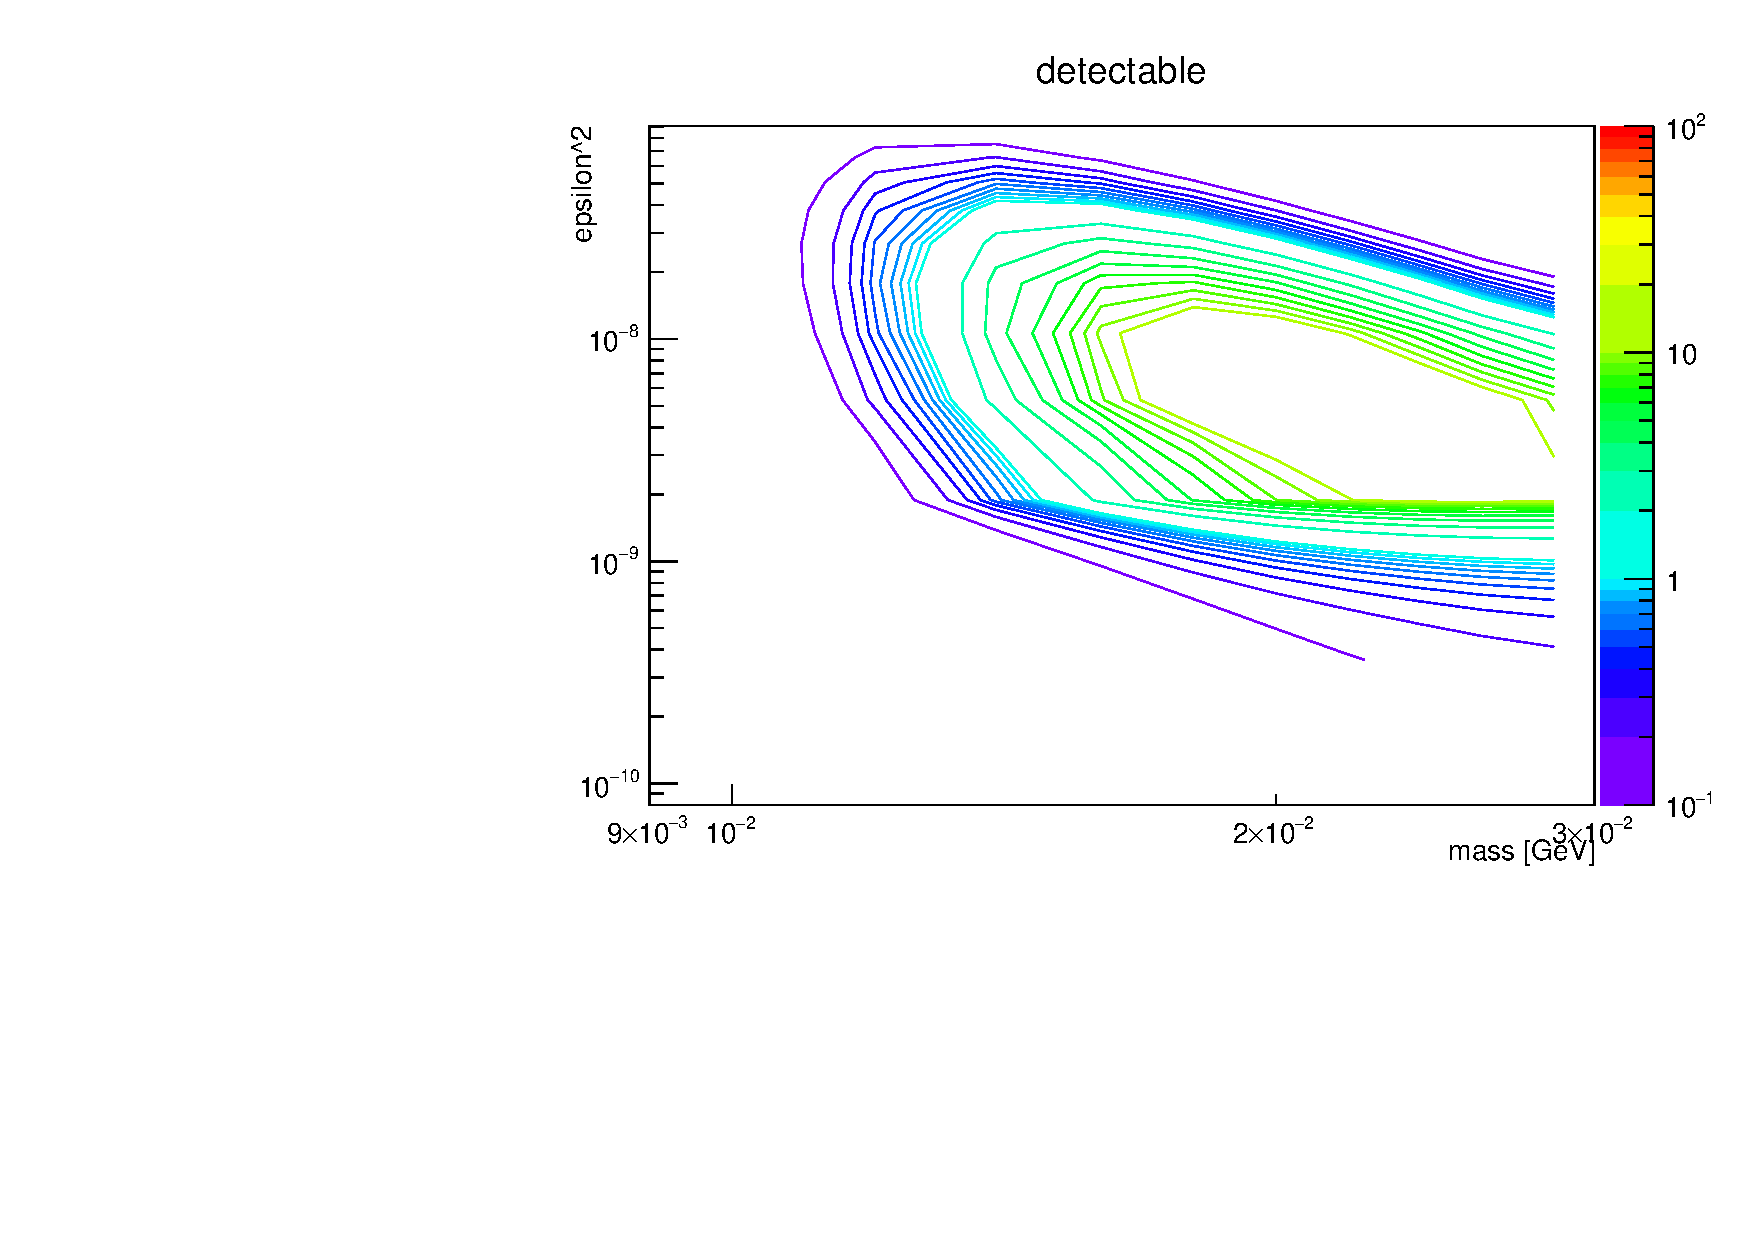
\includegraphics[width=0.7\textwidth,page=1,angle=-90]{vertexing/figs/mgraham_signal}
\end{center}
    \caption{The predicted values of $\mu_{exp}$, the number of detectable heavy photon events expected with $z>z_{cut}$, that were used for the reach estimate in the 2014 proposal.
    The $m_{A'}$ and $\epsilon^2$ ranges, and the binning, are different in this plot compared to other plots in this dissertation.
    The highest contour is at 10 events, and the highest point (at $m_{A'}=22$ MeV, $\epsilon^2=5\times 10^{-9}$) is 17.3 events.
    }
    \label{fig:proposal_detectable}
\end{figure}

The reach projections in the current analysis can be rerun using the trident Monte Carlo sample and some of the proposal assumptions to produce a ``proposal-like'' reach estimate.
A comparison between the proposal and proposal-like estimates is a first step towards understanding any problems with either procedure.
The assumptions for the proposal-like estimate are shown in Table \ref{tab:mc_assumptions}, and the resulting $\mu_{exp}$ is shown in Figure \ref{fig:mc_detectable}.

\begin{table}[ht]
    \begin{center}
        \caption{Assumptions used for the ``proposal-like'' reach estimate.}
        \begin{tabular}{lp{0.5\textwidth}}
            \hline \hline
            Beam energy & 1.056 GeV \\
            Integrated luminosity & 50 nA, 1 week, target thickness 0.116\% $X_0$ \\
            Efficiency dependence on $z$ & Uniform to $z=100$ ($\epsilon_{reco}(m_{A'},z) = \epsilon_{reco}(m_{A'},z_{target})$) \\
            Efficiency at $z_{target}$ & From Monte Carlo \\
            \hline \hline
        \end{tabular}
        \label{tab:mc_assumptions} 
    \end{center}
\end{table}

\begin{figure}[ht]
\begin{center}
    \includegraphics[width=0.7\textwidth,page=16,angle=-90]{vertexing/figs/mc_week_mres_uniform_nosignal_output}
\end{center}
    \caption{Predicted $\mu_{exp}$, the number of detectable heavy photon events expected with $z>z_{cut}$, with the assumptions listed in Table \ref{tab:mc_assumptions}. The highest contour is at 7 events, and the highest point is 7.51 events.}
    \label{fig:mc_detectable}
\end{figure}

The proposal (Figure \ref{fig:proposal_detectable}) and proposal-like (Figure \ref{fig:mc_detectable}) estimates show large differences in $\mu_{exp}$.
The proposal $\mu_{exp}$ has its peak at a lower $m_{A'}$ (22 MeV, as opposed to 28 MeV), and the peak is higher (17.3 events, as opposed to 7 events).
Some differences between Figures \ref{fig:proposal_detectable} and \ref{fig:mc_detectable} are to be expected, since the beam energy and target thickness are different.
However, these differences are of order 10\% and should not produce large changes, or shift the peak $m_{A'}$ by more than the change in the beam energy.
The event selection cuts (and thus the $z_{cut}$) have also changed from the proposal, but not enough to explain the changes seen.

In addition, the low-mass reach in the proposal does not seem plausible: the proposal shows reach at $m_{A'}$ below the lower limit of the HPS acceptance.
The proposal shows exclusion at masses as low as $m_{A'}=14$ MeV, but Monte Carlo samples of low-mass heavy photons show that the efficiency at $z=z_{target}$ falls rapidly in this mass range, from 1\% at $m_{A'}=20$ to 0.06\% at $m_{A'}=16$ MeV, and 0.01\% at $m_{A'}=15$ MeV.
This is expected since the decay products from heavy photons in this mass range are near the minimum opening angle detectable by the SVT; the rate of pairs with reconstructed masses below 15 MeV is still appreciable, but these are mostly pairs with higher masses whose masses were shifted downwards by the mass resolution.

This suggests that the simplified model of the HPS geometric acceptance used for the proposal may have omitted important features of the detector, or that the method used to estimate the detector efficiency may have been flawed.
Further work is needed to identify the problem, and confirm that there is no mistake in the current analysis.
%One possibility of the first type is that the simplified model did not include the effect of the stereo angle on the SVT acceptance.
%Since each module is built by stacking two rectangular half-modules with a small angular offset, the combined acceptance of a HPS SVT module is not rectangular; the stereo sensor dips away from the beam plane on one side.

%The differences in beam energy and target thickness should produce 
%The mass scales should be slightly different 

%I was looking at cross-sections, and it looks like either something is wrong, or recon inefficiency in MC is worse than we thought.
%
%I have 0.6M tridents passing a full set of cuts:
%
%http://www.slac.stanford.edu/~meeg/hps3/users/meeg/vertexing/tails_postfix.pdf
%
%This is on the full set of postTriSummitFixes tritrig, so 0.0682*375 = 25 nb^-1.
%
%So that makes the trident cross-section 23890 nb, which is about a factor of 4 low.
%
%The efficiency of my vertexing cuts is around 50% (which is what you assumed). That gets you halfway, so (assuming your mocked-up acceptance agrees well
%with the trigger acceptance - does it?) it seems like the efficiency to get a V0 is like 50%, which is not great compared to the 0.85^2 that you assumed
%(where did that come from?).
%
%I noticed that the fraction of triggered tritrig events that have at least one V0 is 64%. Of course that includes a lot of low-esum tridents and maybe the
%efficiency moves around, so this is not very conclusive.
